
% Default to the notebook output style

    


% Inherit from the specified cell style.




    
\documentclass[11pt]{article}

    
    
    \usepackage[T1]{fontenc}
    % Nicer default font (+ math font) than Computer Modern for most use cases
    \usepackage{mathpazo}

    % Basic figure setup, for now with no caption control since it's done
    % automatically by Pandoc (which extracts ![](path) syntax from Markdown).
    \usepackage{graphicx}
    % We will generate all images so they have a width \maxwidth. This means
    % that they will get their normal width if they fit onto the page, but
    % are scaled down if they would overflow the margins.
    \makeatletter
    \def\maxwidth{\ifdim\Gin@nat@width>\linewidth\linewidth
    \else\Gin@nat@width\fi}
    \makeatother
    \let\Oldincludegraphics\includegraphics
    % Set max figure width to be 80% of text width, for now hardcoded.
    \renewcommand{\includegraphics}[1]{\Oldincludegraphics[width=.8\maxwidth]{#1}}
    % Ensure that by default, figures have no caption (until we provide a
    % proper Figure object with a Caption API and a way to capture that
    % in the conversion process - todo).
    \usepackage{caption}
    \DeclareCaptionLabelFormat{nolabel}{}
    \captionsetup{labelformat=nolabel}

    \usepackage{adjustbox} % Used to constrain images to a maximum size 
    \usepackage{xcolor} % Allow colors to be defined
    \usepackage{enumerate} % Needed for markdown enumerations to work
    \usepackage{geometry} % Used to adjust the document margins
    \usepackage{amsmath} % Equations
    \usepackage{amssymb} % Equations
    \usepackage{textcomp} % defines textquotesingle
    % Hack from http://tex.stackexchange.com/a/47451/13684:
    \AtBeginDocument{%
        \def\PYZsq{\textquotesingle}% Upright quotes in Pygmentized code
    }
    \usepackage{upquote} % Upright quotes for verbatim code
    \usepackage{eurosym} % defines \euro
    \usepackage[mathletters]{ucs} % Extended unicode (utf-8) support
    \usepackage[utf8x]{inputenc} % Allow utf-8 characters in the tex document
    \usepackage{fancyvrb} % verbatim replacement that allows latex
    \usepackage{grffile} % extends the file name processing of package graphics 
                         % to support a larger range 
    % The hyperref package gives us a pdf with properly built
    % internal navigation ('pdf bookmarks' for the table of contents,
    % internal cross-reference links, web links for URLs, etc.)
    \usepackage{hyperref}
    \usepackage{longtable} % longtable support required by pandoc >1.10
    \usepackage{booktabs}  % table support for pandoc > 1.12.2
    \usepackage[inline]{enumitem} % IRkernel/repr support (it uses the enumerate* environment)
    \usepackage[normalem]{ulem} % ulem is needed to support strikethroughs (\sout)
                                % normalem makes italics be italics, not underlines
    

    
    
    % Colors for the hyperref package
    \definecolor{urlcolor}{rgb}{0,.145,.698}
    \definecolor{linkcolor}{rgb}{.71,0.21,0.01}
    \definecolor{citecolor}{rgb}{.12,.54,.11}

    % ANSI colors
    \definecolor{ansi-black}{HTML}{3E424D}
    \definecolor{ansi-black-intense}{HTML}{282C36}
    \definecolor{ansi-red}{HTML}{E75C58}
    \definecolor{ansi-red-intense}{HTML}{B22B31}
    \definecolor{ansi-green}{HTML}{00A250}
    \definecolor{ansi-green-intense}{HTML}{007427}
    \definecolor{ansi-yellow}{HTML}{DDB62B}
    \definecolor{ansi-yellow-intense}{HTML}{B27D12}
    \definecolor{ansi-blue}{HTML}{208FFB}
    \definecolor{ansi-blue-intense}{HTML}{0065CA}
    \definecolor{ansi-magenta}{HTML}{D160C4}
    \definecolor{ansi-magenta-intense}{HTML}{A03196}
    \definecolor{ansi-cyan}{HTML}{60C6C8}
    \definecolor{ansi-cyan-intense}{HTML}{258F8F}
    \definecolor{ansi-white}{HTML}{C5C1B4}
    \definecolor{ansi-white-intense}{HTML}{A1A6B2}

    % commands and environments needed by pandoc snippets
    % extracted from the output of `pandoc -s`
    \providecommand{\tightlist}{%
      \setlength{\itemsep}{0pt}\setlength{\parskip}{0pt}}
    \DefineVerbatimEnvironment{Highlighting}{Verbatim}{commandchars=\\\{\}}
    % Add ',fontsize=\small' for more characters per line
    \newenvironment{Shaded}{}{}
    \newcommand{\KeywordTok}[1]{\textcolor[rgb]{0.00,0.44,0.13}{\textbf{{#1}}}}
    \newcommand{\DataTypeTok}[1]{\textcolor[rgb]{0.56,0.13,0.00}{{#1}}}
    \newcommand{\DecValTok}[1]{\textcolor[rgb]{0.25,0.63,0.44}{{#1}}}
    \newcommand{\BaseNTok}[1]{\textcolor[rgb]{0.25,0.63,0.44}{{#1}}}
    \newcommand{\FloatTok}[1]{\textcolor[rgb]{0.25,0.63,0.44}{{#1}}}
    \newcommand{\CharTok}[1]{\textcolor[rgb]{0.25,0.44,0.63}{{#1}}}
    \newcommand{\StringTok}[1]{\textcolor[rgb]{0.25,0.44,0.63}{{#1}}}
    \newcommand{\CommentTok}[1]{\textcolor[rgb]{0.38,0.63,0.69}{\textit{{#1}}}}
    \newcommand{\OtherTok}[1]{\textcolor[rgb]{0.00,0.44,0.13}{{#1}}}
    \newcommand{\AlertTok}[1]{\textcolor[rgb]{1.00,0.00,0.00}{\textbf{{#1}}}}
    \newcommand{\FunctionTok}[1]{\textcolor[rgb]{0.02,0.16,0.49}{{#1}}}
    \newcommand{\RegionMarkerTok}[1]{{#1}}
    \newcommand{\ErrorTok}[1]{\textcolor[rgb]{1.00,0.00,0.00}{\textbf{{#1}}}}
    \newcommand{\NormalTok}[1]{{#1}}
    
    % Additional commands for more recent versions of Pandoc
    \newcommand{\ConstantTok}[1]{\textcolor[rgb]{0.53,0.00,0.00}{{#1}}}
    \newcommand{\SpecialCharTok}[1]{\textcolor[rgb]{0.25,0.44,0.63}{{#1}}}
    \newcommand{\VerbatimStringTok}[1]{\textcolor[rgb]{0.25,0.44,0.63}{{#1}}}
    \newcommand{\SpecialStringTok}[1]{\textcolor[rgb]{0.73,0.40,0.53}{{#1}}}
    \newcommand{\ImportTok}[1]{{#1}}
    \newcommand{\DocumentationTok}[1]{\textcolor[rgb]{0.73,0.13,0.13}{\textit{{#1}}}}
    \newcommand{\AnnotationTok}[1]{\textcolor[rgb]{0.38,0.63,0.69}{\textbf{\textit{{#1}}}}}
    \newcommand{\CommentVarTok}[1]{\textcolor[rgb]{0.38,0.63,0.69}{\textbf{\textit{{#1}}}}}
    \newcommand{\VariableTok}[1]{\textcolor[rgb]{0.10,0.09,0.49}{{#1}}}
    \newcommand{\ControlFlowTok}[1]{\textcolor[rgb]{0.00,0.44,0.13}{\textbf{{#1}}}}
    \newcommand{\OperatorTok}[1]{\textcolor[rgb]{0.40,0.40,0.40}{{#1}}}
    \newcommand{\BuiltInTok}[1]{{#1}}
    \newcommand{\ExtensionTok}[1]{{#1}}
    \newcommand{\PreprocessorTok}[1]{\textcolor[rgb]{0.74,0.48,0.00}{{#1}}}
    \newcommand{\AttributeTok}[1]{\textcolor[rgb]{0.49,0.56,0.16}{{#1}}}
    \newcommand{\InformationTok}[1]{\textcolor[rgb]{0.38,0.63,0.69}{\textbf{\textit{{#1}}}}}
    \newcommand{\WarningTok}[1]{\textcolor[rgb]{0.38,0.63,0.69}{\textbf{\textit{{#1}}}}}
    
    
    % Define a nice break command that doesn't care if a line doesn't already
    % exist.
    \def\br{\hspace*{\fill} \\* }
    % Math Jax compatability definitions
    \def\gt{>}
    \def\lt{<}
    % Document parameters
    \title{HW2}
    
    
    

    % Pygments definitions
    
\makeatletter
\def\PY@reset{\let\PY@it=\relax \let\PY@bf=\relax%
    \let\PY@ul=\relax \let\PY@tc=\relax%
    \let\PY@bc=\relax \let\PY@ff=\relax}
\def\PY@tok#1{\csname PY@tok@#1\endcsname}
\def\PY@toks#1+{\ifx\relax#1\empty\else%
    \PY@tok{#1}\expandafter\PY@toks\fi}
\def\PY@do#1{\PY@bc{\PY@tc{\PY@ul{%
    \PY@it{\PY@bf{\PY@ff{#1}}}}}}}
\def\PY#1#2{\PY@reset\PY@toks#1+\relax+\PY@do{#2}}

\expandafter\def\csname PY@tok@w\endcsname{\def\PY@tc##1{\textcolor[rgb]{0.73,0.73,0.73}{##1}}}
\expandafter\def\csname PY@tok@c\endcsname{\let\PY@it=\textit\def\PY@tc##1{\textcolor[rgb]{0.25,0.50,0.50}{##1}}}
\expandafter\def\csname PY@tok@cp\endcsname{\def\PY@tc##1{\textcolor[rgb]{0.74,0.48,0.00}{##1}}}
\expandafter\def\csname PY@tok@k\endcsname{\let\PY@bf=\textbf\def\PY@tc##1{\textcolor[rgb]{0.00,0.50,0.00}{##1}}}
\expandafter\def\csname PY@tok@kp\endcsname{\def\PY@tc##1{\textcolor[rgb]{0.00,0.50,0.00}{##1}}}
\expandafter\def\csname PY@tok@kt\endcsname{\def\PY@tc##1{\textcolor[rgb]{0.69,0.00,0.25}{##1}}}
\expandafter\def\csname PY@tok@o\endcsname{\def\PY@tc##1{\textcolor[rgb]{0.40,0.40,0.40}{##1}}}
\expandafter\def\csname PY@tok@ow\endcsname{\let\PY@bf=\textbf\def\PY@tc##1{\textcolor[rgb]{0.67,0.13,1.00}{##1}}}
\expandafter\def\csname PY@tok@nb\endcsname{\def\PY@tc##1{\textcolor[rgb]{0.00,0.50,0.00}{##1}}}
\expandafter\def\csname PY@tok@nf\endcsname{\def\PY@tc##1{\textcolor[rgb]{0.00,0.00,1.00}{##1}}}
\expandafter\def\csname PY@tok@nc\endcsname{\let\PY@bf=\textbf\def\PY@tc##1{\textcolor[rgb]{0.00,0.00,1.00}{##1}}}
\expandafter\def\csname PY@tok@nn\endcsname{\let\PY@bf=\textbf\def\PY@tc##1{\textcolor[rgb]{0.00,0.00,1.00}{##1}}}
\expandafter\def\csname PY@tok@ne\endcsname{\let\PY@bf=\textbf\def\PY@tc##1{\textcolor[rgb]{0.82,0.25,0.23}{##1}}}
\expandafter\def\csname PY@tok@nv\endcsname{\def\PY@tc##1{\textcolor[rgb]{0.10,0.09,0.49}{##1}}}
\expandafter\def\csname PY@tok@no\endcsname{\def\PY@tc##1{\textcolor[rgb]{0.53,0.00,0.00}{##1}}}
\expandafter\def\csname PY@tok@nl\endcsname{\def\PY@tc##1{\textcolor[rgb]{0.63,0.63,0.00}{##1}}}
\expandafter\def\csname PY@tok@ni\endcsname{\let\PY@bf=\textbf\def\PY@tc##1{\textcolor[rgb]{0.60,0.60,0.60}{##1}}}
\expandafter\def\csname PY@tok@na\endcsname{\def\PY@tc##1{\textcolor[rgb]{0.49,0.56,0.16}{##1}}}
\expandafter\def\csname PY@tok@nt\endcsname{\let\PY@bf=\textbf\def\PY@tc##1{\textcolor[rgb]{0.00,0.50,0.00}{##1}}}
\expandafter\def\csname PY@tok@nd\endcsname{\def\PY@tc##1{\textcolor[rgb]{0.67,0.13,1.00}{##1}}}
\expandafter\def\csname PY@tok@s\endcsname{\def\PY@tc##1{\textcolor[rgb]{0.73,0.13,0.13}{##1}}}
\expandafter\def\csname PY@tok@sd\endcsname{\let\PY@it=\textit\def\PY@tc##1{\textcolor[rgb]{0.73,0.13,0.13}{##1}}}
\expandafter\def\csname PY@tok@si\endcsname{\let\PY@bf=\textbf\def\PY@tc##1{\textcolor[rgb]{0.73,0.40,0.53}{##1}}}
\expandafter\def\csname PY@tok@se\endcsname{\let\PY@bf=\textbf\def\PY@tc##1{\textcolor[rgb]{0.73,0.40,0.13}{##1}}}
\expandafter\def\csname PY@tok@sr\endcsname{\def\PY@tc##1{\textcolor[rgb]{0.73,0.40,0.53}{##1}}}
\expandafter\def\csname PY@tok@ss\endcsname{\def\PY@tc##1{\textcolor[rgb]{0.10,0.09,0.49}{##1}}}
\expandafter\def\csname PY@tok@sx\endcsname{\def\PY@tc##1{\textcolor[rgb]{0.00,0.50,0.00}{##1}}}
\expandafter\def\csname PY@tok@m\endcsname{\def\PY@tc##1{\textcolor[rgb]{0.40,0.40,0.40}{##1}}}
\expandafter\def\csname PY@tok@gh\endcsname{\let\PY@bf=\textbf\def\PY@tc##1{\textcolor[rgb]{0.00,0.00,0.50}{##1}}}
\expandafter\def\csname PY@tok@gu\endcsname{\let\PY@bf=\textbf\def\PY@tc##1{\textcolor[rgb]{0.50,0.00,0.50}{##1}}}
\expandafter\def\csname PY@tok@gd\endcsname{\def\PY@tc##1{\textcolor[rgb]{0.63,0.00,0.00}{##1}}}
\expandafter\def\csname PY@tok@gi\endcsname{\def\PY@tc##1{\textcolor[rgb]{0.00,0.63,0.00}{##1}}}
\expandafter\def\csname PY@tok@gr\endcsname{\def\PY@tc##1{\textcolor[rgb]{1.00,0.00,0.00}{##1}}}
\expandafter\def\csname PY@tok@ge\endcsname{\let\PY@it=\textit}
\expandafter\def\csname PY@tok@gs\endcsname{\let\PY@bf=\textbf}
\expandafter\def\csname PY@tok@gp\endcsname{\let\PY@bf=\textbf\def\PY@tc##1{\textcolor[rgb]{0.00,0.00,0.50}{##1}}}
\expandafter\def\csname PY@tok@go\endcsname{\def\PY@tc##1{\textcolor[rgb]{0.53,0.53,0.53}{##1}}}
\expandafter\def\csname PY@tok@gt\endcsname{\def\PY@tc##1{\textcolor[rgb]{0.00,0.27,0.87}{##1}}}
\expandafter\def\csname PY@tok@err\endcsname{\def\PY@bc##1{\setlength{\fboxsep}{0pt}\fcolorbox[rgb]{1.00,0.00,0.00}{1,1,1}{\strut ##1}}}
\expandafter\def\csname PY@tok@kc\endcsname{\let\PY@bf=\textbf\def\PY@tc##1{\textcolor[rgb]{0.00,0.50,0.00}{##1}}}
\expandafter\def\csname PY@tok@kd\endcsname{\let\PY@bf=\textbf\def\PY@tc##1{\textcolor[rgb]{0.00,0.50,0.00}{##1}}}
\expandafter\def\csname PY@tok@kn\endcsname{\let\PY@bf=\textbf\def\PY@tc##1{\textcolor[rgb]{0.00,0.50,0.00}{##1}}}
\expandafter\def\csname PY@tok@kr\endcsname{\let\PY@bf=\textbf\def\PY@tc##1{\textcolor[rgb]{0.00,0.50,0.00}{##1}}}
\expandafter\def\csname PY@tok@bp\endcsname{\def\PY@tc##1{\textcolor[rgb]{0.00,0.50,0.00}{##1}}}
\expandafter\def\csname PY@tok@fm\endcsname{\def\PY@tc##1{\textcolor[rgb]{0.00,0.00,1.00}{##1}}}
\expandafter\def\csname PY@tok@vc\endcsname{\def\PY@tc##1{\textcolor[rgb]{0.10,0.09,0.49}{##1}}}
\expandafter\def\csname PY@tok@vg\endcsname{\def\PY@tc##1{\textcolor[rgb]{0.10,0.09,0.49}{##1}}}
\expandafter\def\csname PY@tok@vi\endcsname{\def\PY@tc##1{\textcolor[rgb]{0.10,0.09,0.49}{##1}}}
\expandafter\def\csname PY@tok@vm\endcsname{\def\PY@tc##1{\textcolor[rgb]{0.10,0.09,0.49}{##1}}}
\expandafter\def\csname PY@tok@sa\endcsname{\def\PY@tc##1{\textcolor[rgb]{0.73,0.13,0.13}{##1}}}
\expandafter\def\csname PY@tok@sb\endcsname{\def\PY@tc##1{\textcolor[rgb]{0.73,0.13,0.13}{##1}}}
\expandafter\def\csname PY@tok@sc\endcsname{\def\PY@tc##1{\textcolor[rgb]{0.73,0.13,0.13}{##1}}}
\expandafter\def\csname PY@tok@dl\endcsname{\def\PY@tc##1{\textcolor[rgb]{0.73,0.13,0.13}{##1}}}
\expandafter\def\csname PY@tok@s2\endcsname{\def\PY@tc##1{\textcolor[rgb]{0.73,0.13,0.13}{##1}}}
\expandafter\def\csname PY@tok@sh\endcsname{\def\PY@tc##1{\textcolor[rgb]{0.73,0.13,0.13}{##1}}}
\expandafter\def\csname PY@tok@s1\endcsname{\def\PY@tc##1{\textcolor[rgb]{0.73,0.13,0.13}{##1}}}
\expandafter\def\csname PY@tok@mb\endcsname{\def\PY@tc##1{\textcolor[rgb]{0.40,0.40,0.40}{##1}}}
\expandafter\def\csname PY@tok@mf\endcsname{\def\PY@tc##1{\textcolor[rgb]{0.40,0.40,0.40}{##1}}}
\expandafter\def\csname PY@tok@mh\endcsname{\def\PY@tc##1{\textcolor[rgb]{0.40,0.40,0.40}{##1}}}
\expandafter\def\csname PY@tok@mi\endcsname{\def\PY@tc##1{\textcolor[rgb]{0.40,0.40,0.40}{##1}}}
\expandafter\def\csname PY@tok@il\endcsname{\def\PY@tc##1{\textcolor[rgb]{0.40,0.40,0.40}{##1}}}
\expandafter\def\csname PY@tok@mo\endcsname{\def\PY@tc##1{\textcolor[rgb]{0.40,0.40,0.40}{##1}}}
\expandafter\def\csname PY@tok@ch\endcsname{\let\PY@it=\textit\def\PY@tc##1{\textcolor[rgb]{0.25,0.50,0.50}{##1}}}
\expandafter\def\csname PY@tok@cm\endcsname{\let\PY@it=\textit\def\PY@tc##1{\textcolor[rgb]{0.25,0.50,0.50}{##1}}}
\expandafter\def\csname PY@tok@cpf\endcsname{\let\PY@it=\textit\def\PY@tc##1{\textcolor[rgb]{0.25,0.50,0.50}{##1}}}
\expandafter\def\csname PY@tok@c1\endcsname{\let\PY@it=\textit\def\PY@tc##1{\textcolor[rgb]{0.25,0.50,0.50}{##1}}}
\expandafter\def\csname PY@tok@cs\endcsname{\let\PY@it=\textit\def\PY@tc##1{\textcolor[rgb]{0.25,0.50,0.50}{##1}}}

\def\PYZbs{\char`\\}
\def\PYZus{\char`\_}
\def\PYZob{\char`\{}
\def\PYZcb{\char`\}}
\def\PYZca{\char`\^}
\def\PYZam{\char`\&}
\def\PYZlt{\char`\<}
\def\PYZgt{\char`\>}
\def\PYZsh{\char`\#}
\def\PYZpc{\char`\%}
\def\PYZdl{\char`\$}
\def\PYZhy{\char`\-}
\def\PYZsq{\char`\'}
\def\PYZdq{\char`\"}
\def\PYZti{\char`\~}
% for compatibility with earlier versions
\def\PYZat{@}
\def\PYZlb{[}
\def\PYZrb{]}
\makeatother


    % Exact colors from NB
    \definecolor{incolor}{rgb}{0.0, 0.0, 0.5}
    \definecolor{outcolor}{rgb}{0.545, 0.0, 0.0}



    
    % Prevent overflowing lines due to hard-to-break entities
    \sloppy 
    % Setup hyperref package
    \hypersetup{
      breaklinks=true,  % so long urls are correctly broken across lines
      colorlinks=true,
      urlcolor=urlcolor,
      linkcolor=linkcolor,
      citecolor=citecolor,
      }
    % Slightly bigger margins than the latex defaults
    
    \geometry{verbose,tmargin=1in,bmargin=1in,lmargin=1in,rmargin=1in}
    
    

    \begin{document}
    
    
    \maketitle
    
    

    
    \section{CSE 152: Intro to Computer Vision - Spring 2019 Assignment
2}\label{cse-152-intro-to-computer-vision---spring-2019-assignment-2}

\subsection{Instructor: David Kriegman}\label{instructor-david-kriegman}

\subsubsection{Assignment published on Friday, April 26,
2019}\label{assignment-published-on-friday-april-26-2019}

\subsubsection{Due on Wednesday, May 8, 2019 at
11:59pm}\label{due-on-wednesday-may-8-2019-at-1159pm}

\subsection{Instructions}\label{instructions}

\begin{itemize}
\tightlist
\item
  This assignment must be completed individually. Review the academic
  integrity and collaboration policies on the course website.
\item
  All solutions should be written in this notebook.
\item
  If you want to modify the skeleton code, you may do so. It has been
  merely been provided as a framework for your solution.
\item
  You may use Python packages for basic linear algebra (e.g. NumPy or
  SciPy for basic operations), but you may not use packages that
  directly solve the problem. If you are unsure about using a specific
  package or function, ask the instructor and/or teaching assistants for
  clarification.
\item
  You must submit this notebook exported as a PDF. You must also submit
  this notebook as an \texttt{.ipynb} file. Submit both files
  (\texttt{.pdf} and \texttt{.ipynb}) on Gradescope. \textbf{You must
  mark the PDF pages associated with each question in Gradescope. If you
  fail to do so, we may dock points.}
\item
  It is highly recommended that you begin working on this assignment
  early.
\item
  \textbf{Late policy:} a penalty of 10\% per day after the due date.
\end{itemize}

\begin{center}\rule{0.5\linewidth}{\linethickness}\end{center}

    \subsection{Problem 1: Stereo and Disparity {[}3
pts{]}}\label{problem-1-stereo-and-disparity-3-pts}

Consider two cameras whose (virtual) image planes are the z=1 plane, and
whose focal points are at (-20, 0, 0) and (20, 0, 0). We''ll call a
point in the first camera (x, y), and a point in the second camera (u,
v). Points in each camera are relative to the camera center. So, for
example if (x, y) = (0, 0), this is really the point (-20, 0, 1) in
world coordinates, while if (u, v) = (0, 0) this is the point (20, 0,
1).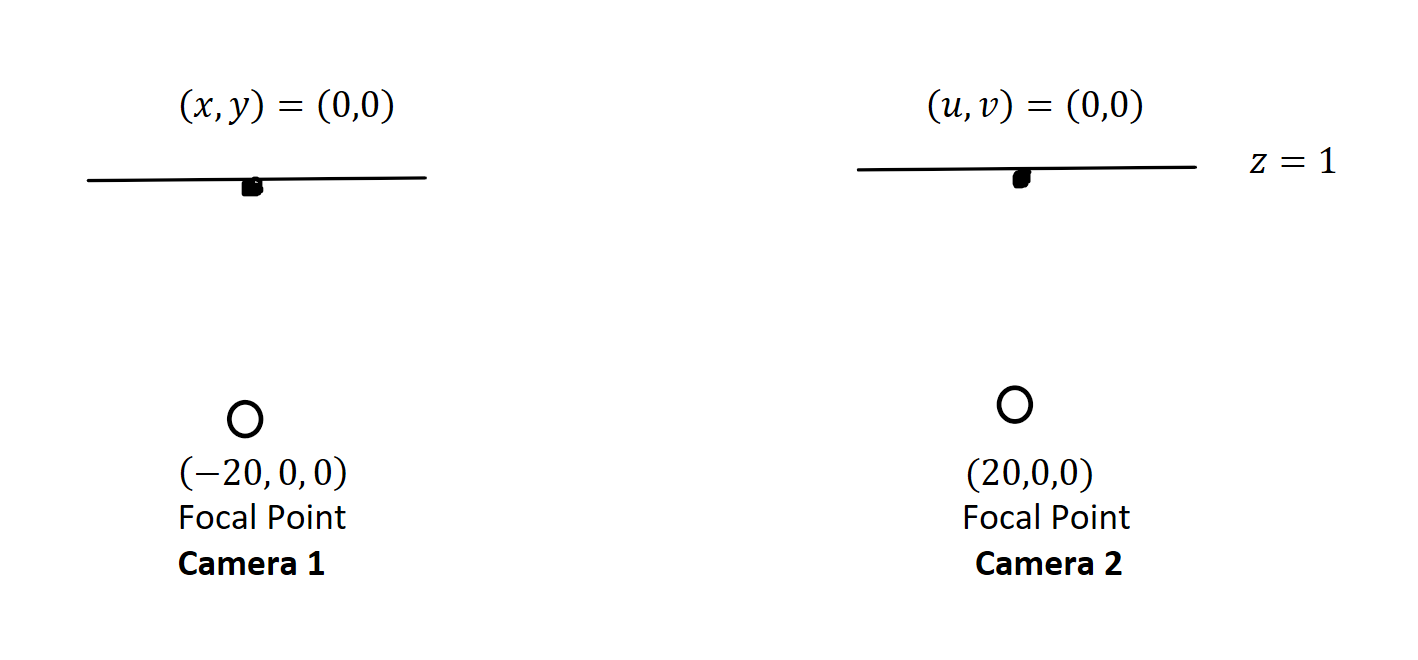
\includegraphics{fig/fig1.png} a) Suppose the points (x, y) = (12,
12) is matched to the point (u, v) = (1, 12). What is the 3D location of
this point?

\begin{enumerate}
\def\labelenumi{\alph{enumi})}
\setcounter{enumi}{1}
\tightlist
\item
  Consider points that lie on the line x + z = 0, y = 0. Use the same
  stereo setup as before. Write an analytic expression giving the
  disparity of a point on this line after it projects onto the two
  images, as a function of its position in the right image. So your
  expression should only involve the variables u and d (for disparity).
  Your expression only needs to be valid for points on the line that are
  in front of the cameras, i.e. with z \textgreater{} 1.
\end{enumerate}

    A). We have that: Baseline d = 40 Focal Length f = 1 (x, y) = (12, 12)
(u, v) = (1 , 12)

\begin{verbatim}
X = d * f * x / (x - u)         A displacement of -20 should be added since the equation 
  = (40 * 1 * 12) / (12 - 1)    assumes camera 1 is located at the origin where as in 
  = 480 / 11                    this set up it is actually located at (-20, 0, 0)
X = X - 20
  = 260 / 11

Z = d * f / (x - u)
  = (40 * 1) / (12 - 1)
  = 40 / 11
  
Y = z/f * y
  = (40/ 11) / 1 * 12
  = 480 / 11
  
(X, Y, Z) = 1/11 (260, 480, 40)
\end{verbatim}

B). Since Y is a constant value 0, we do not have to worry about the
Y-disparity Let I be the X value used to calculate x and y, so I = X +
20 (due to the -20 offset of camera 1 from the origin) Let J be the Z
value used to calculate x and y. Let b be the length of the baseline, so
b = 40 Let f be the focal length, so f = 1

\begin{verbatim}
We have the formulas-

    x = f * (I / J),     u = f * ((I - b)/ J),    d = x - u
We can substitute and expand:

    d = x - u
      = f * (I / J) - f * ((I - b)/ J)       , f = 1
      = (I / J) - (I - 40)/ J
      = X/J + 20/J - X/J - 20/J + 40/J       , J = Z
      = 40/Z
      
\end{verbatim}

We must put 40/Z in terms of u, we have that:

\begin{verbatim}
    -2u = -2 ((I-b)/J)
        = -2 (X/Z + 20/Z -b/Z)               , we know that X = -Z since X + Y = 0
        = -2 (-1 + 20/Z - b/Z)
        = 2 - 40/Z + 2b/Z                    , we know that b = 40
        = 2 + b/Z
    b/Z = 40/Z = -2 - 2u
    
\end{verbatim}

Therefore we have the overall formula:

\begin{verbatim}
    d = -2 -2u
    
\end{verbatim}

    \subsection{Problem 2: Sparse Stereo Matching {[}20
pts{]}}\label{problem-2-sparse-stereo-matching-20-pts}

    In this problem we will play around with sparse stereo matching methods.
You will work on two image pairs, a warrior figure and a figure from the
Matrix movies. These files both contain two images, two camera matrices,
and associated sets of corresponding points (extracted by manually
clicking the images).

For the problems below, you will complete functions to demonstrate
results on warrior image pairs (warrior1.png, warrior2.png). In all
cases, you should apply the same procedures on the matrix image pair
(matrix1.png, matrix2.png) as well. (Provide the same thing for BOTH
matrix and warrior.) Note that the matrix image pair is harder, in the
sense that matching algorithms will not work quite as well on it. You
should expect good results, however, on warrior.

    \begin{Verbatim}[commandchars=\\\{\}]
{\color{incolor}In [{\color{incolor}9}]:} \PY{k+kn}{import} \PY{n+nn}{numpy} \PY{k}{as} \PY{n+nn}{np}
        \PY{k+kn}{import} \PY{n+nn}{matplotlib}\PY{n+nn}{.}\PY{n+nn}{pyplot} \PY{k}{as} \PY{n+nn}{plt}
        \PY{k+kn}{from} \PY{n+nn}{skimage} \PY{k}{import} \PY{n}{io}
\end{Verbatim}


    \begin{Verbatim}[commandchars=\\\{\}]
{\color{incolor}In [{\color{incolor}10}]:} \PY{k}{def} \PY{n+nf}{rgb2gray}\PY{p}{(}\PY{n}{rgb}\PY{p}{)}\PY{p}{:}
             \PY{l+s+sd}{\PYZdq{}\PYZdq{}\PYZdq{} Convert rgb image to grayscale.}
         \PY{l+s+sd}{    \PYZdq{}\PYZdq{}\PYZdq{}}
             \PY{k}{return} \PY{n}{np}\PY{o}{.}\PY{n}{dot}\PY{p}{(}\PY{n}{rgb}\PY{p}{[}\PY{o}{.}\PY{o}{.}\PY{o}{.}\PY{p}{,}\PY{p}{:}\PY{l+m+mi}{3}\PY{p}{]}\PY{p}{,} \PY{p}{[}\PY{l+m+mf}{0.299}\PY{p}{,} \PY{l+m+mf}{0.587}\PY{p}{,} \PY{l+m+mf}{0.114}\PY{p}{]}\PY{p}{)}
         
         \PY{c+c1}{\PYZsh{} convert points from euclidean to homogeneous}
         \PY{k}{def} \PY{n+nf}{to\PYZus{}homog}\PY{p}{(}\PY{n}{points}\PY{p}{)}\PY{p}{:}
             \PY{n}{points} \PY{o}{=} \PY{n}{np}\PY{o}{.}\PY{n}{concatenate}\PY{p}{(}\PY{p}{(}\PY{n}{points}\PY{p}{,} \PY{n}{np}\PY{o}{.}\PY{n}{ones}\PY{p}{(}\PY{p}{(}\PY{l+m+mi}{1}\PY{p}{,} \PY{n}{points}\PY{o}{.}\PY{n}{shape}\PY{p}{[}\PY{l+m+mi}{1}\PY{p}{]}\PY{p}{)}\PY{p}{)}\PY{p}{)}\PY{p}{,} \PY{n}{axis}\PY{o}{=}\PY{l+m+mi}{0}\PY{p}{)}
             \PY{k}{return} \PY{n}{points}
         
         \PY{c+c1}{\PYZsh{} convert points from homogeneous to euclidean}
         \PY{k}{def} \PY{n+nf}{from\PYZus{}homog}\PY{p}{(}\PY{n}{points\PYZus{}homog}\PY{p}{)}\PY{p}{:}
             \PY{n}{z} \PY{o}{=} \PY{n}{points\PYZus{}homog}\PY{p}{[}\PY{o}{\PYZhy{}}\PY{l+m+mi}{1}\PY{p}{,}\PY{p}{:}\PY{p}{]}
             \PY{n}{points\PYZus{}homog} \PY{o}{=} \PY{n}{points\PYZus{}homog}\PY{p}{[}\PY{p}{:}\PY{l+m+mi}{2}\PY{p}{,}\PY{p}{:}\PY{p}{]}\PY{o}{/}\PY{n}{z}
             \PY{k}{return} \PY{n}{points\PYZus{}homog}
\end{Verbatim}


    \begin{Verbatim}[commandchars=\\\{\}]
{\color{incolor}In [{\color{incolor}11}]:} \PY{c+c1}{\PYZsh{} plot matching result}
         \PY{k}{def} \PY{n+nf}{show\PYZus{}matching\PYZus{}result}\PY{p}{(}\PY{n}{img1}\PY{p}{,} \PY{n}{img2}\PY{p}{,} \PY{n}{matching}\PY{p}{)}\PY{p}{:}
             \PY{n}{fig} \PY{o}{=} \PY{n}{plt}\PY{o}{.}\PY{n}{figure}\PY{p}{(}\PY{n}{figsize}\PY{o}{=}\PY{p}{(}\PY{l+m+mi}{20}\PY{p}{,} \PY{l+m+mi}{20}\PY{p}{)}\PY{p}{)}
             \PY{n}{plt}\PY{o}{.}\PY{n}{imshow}\PY{p}{(}\PY{n}{np}\PY{o}{.}\PY{n}{hstack}\PY{p}{(}\PY{p}{(}\PY{n}{img1}\PY{p}{,} \PY{n}{img2}\PY{p}{)}\PY{p}{)}\PY{p}{,} \PY{n}{cmap}\PY{o}{=}\PY{l+s+s1}{\PYZsq{}}\PY{l+s+s1}{gray}\PY{l+s+s1}{\PYZsq{}}\PY{p}{)} \PY{c+c1}{\PYZsh{} two dino images are of different sizes, resize one before use}
             \PY{k}{for} \PY{n}{p1}\PY{p}{,} \PY{n}{p2} \PY{o+ow}{in} \PY{n}{matching}\PY{p}{:}
                 \PY{n}{plt}\PY{o}{.}\PY{n}{scatter}\PY{p}{(}\PY{n}{p1}\PY{p}{[}\PY{l+m+mi}{0}\PY{p}{]}\PY{p}{,} \PY{n}{p1}\PY{p}{[}\PY{l+m+mi}{1}\PY{p}{]}\PY{p}{,} \PY{n}{s}\PY{o}{=}\PY{l+m+mi}{35}\PY{p}{,} \PY{n}{edgecolors}\PY{o}{=}\PY{l+s+s1}{\PYZsq{}}\PY{l+s+s1}{r}\PY{l+s+s1}{\PYZsq{}}\PY{p}{,} \PY{n}{facecolors}\PY{o}{=}\PY{l+s+s1}{\PYZsq{}}\PY{l+s+s1}{none}\PY{l+s+s1}{\PYZsq{}}\PY{p}{)}
                 \PY{n}{plt}\PY{o}{.}\PY{n}{scatter}\PY{p}{(}\PY{n}{p2}\PY{p}{[}\PY{l+m+mi}{0}\PY{p}{]} \PY{o}{+} \PY{n}{img1}\PY{o}{.}\PY{n}{shape}\PY{p}{[}\PY{l+m+mi}{1}\PY{p}{]}\PY{p}{,} \PY{n}{p2}\PY{p}{[}\PY{l+m+mi}{1}\PY{p}{]}\PY{p}{,} \PY{n}{s}\PY{o}{=}\PY{l+m+mi}{35}\PY{p}{,} \PY{n}{edgecolors}\PY{o}{=}\PY{l+s+s1}{\PYZsq{}}\PY{l+s+s1}{r}\PY{l+s+s1}{\PYZsq{}}\PY{p}{,} \PY{n}{facecolors}\PY{o}{=}\PY{l+s+s1}{\PYZsq{}}\PY{l+s+s1}{none}\PY{l+s+s1}{\PYZsq{}}\PY{p}{)}
                 \PY{n}{plt}\PY{o}{.}\PY{n}{plot}\PY{p}{(}\PY{p}{[}\PY{n}{p1}\PY{p}{[}\PY{l+m+mi}{0}\PY{p}{]}\PY{p}{,} \PY{n}{p2}\PY{p}{[}\PY{l+m+mi}{0}\PY{p}{]} \PY{o}{+} \PY{n}{img1}\PY{o}{.}\PY{n}{shape}\PY{p}{[}\PY{l+m+mi}{1}\PY{p}{]}\PY{p}{]}\PY{p}{,} \PY{p}{[}\PY{n}{p1}\PY{p}{[}\PY{l+m+mi}{1}\PY{p}{]}\PY{p}{,} \PY{n}{p2}\PY{p}{[}\PY{l+m+mi}{1}\PY{p}{]}\PY{p}{]}\PY{p}{)}
             \PY{n}{plt}\PY{o}{.}\PY{n}{show}\PY{p}{(}\PY{p}{)}
\end{Verbatim}


    \subsubsection{Epipolar Geometry}\label{epipolar-geometry}

Using the fundamental\_matrix function and the corresponding points
provided in cor1.npy and cor2.npy, calculate the fundamental matrix.
Note that estimation of the fundamental matrix is ill-conditioned; we
need to normalize coordinates before computing the fundamental matrix in
order to remedy this problem. The fundamental\_matrix function contains
code for normalization, so you just need to complete the
compute\_fundamental function by implementing the eight-point algorithm.

Next, use this fundamental matrix, implement plot\_epipolar\_lines to
plot the epipolar lines in both image pairs. For this part you may want
to complete the function compute\_fundamental and then use
plot\_epipolar\_lines to draw epipolar lines on both images. Below, we
provide some example results on the dino image pair. Your results should
look similar. Include your results for matrix and warrior as per the
figure below. 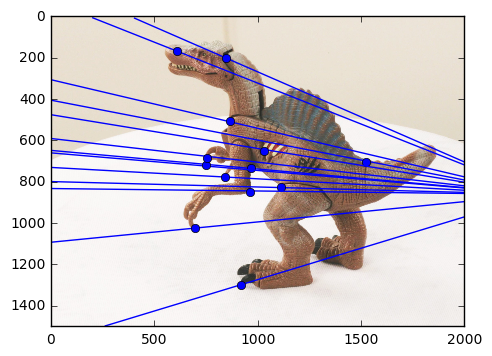
\includegraphics{fig/dinoEpi1.png}
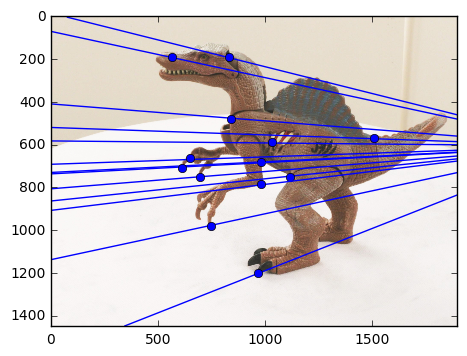
\includegraphics{fig/dinoEpi2.png}

    \begin{Verbatim}[commandchars=\\\{\}]
{\color{incolor}In [{\color{incolor}12}]:} \PY{k+kn}{import} \PY{n+nn}{numpy} \PY{k}{as} \PY{n+nn}{np}
         \PY{k+kn}{import} \PY{n+nn}{matplotlib}\PY{n+nn}{.}\PY{n+nn}{pyplot} \PY{k}{as} \PY{n+nn}{plt}
         
         \PY{n}{imgs} \PY{o}{=} \PY{p}{[}\PY{p}{]}
         \PY{k}{for} \PY{n}{i} \PY{o+ow}{in} \PY{n+nb}{range}\PY{p}{(}\PY{l+m+mi}{2}\PY{p}{)}\PY{p}{:}
             \PY{n}{img} \PY{o}{=} \PY{n}{io}\PY{o}{.}\PY{n}{imread}\PY{p}{(}\PY{l+s+s1}{\PYZsq{}}\PY{l+s+s1}{p4/warrior/warrior}\PY{l+s+s1}{\PYZsq{}} \PY{o}{+} \PY{n+nb}{str}\PY{p}{(}\PY{n}{i}\PY{p}{)} \PY{o}{+} \PY{l+s+s1}{\PYZsq{}}\PY{l+s+s1}{.png}\PY{l+s+s1}{\PYZsq{}}\PY{p}{)}
             \PY{c+c1}{\PYZsh{}img = io.imread(\PYZsq{}p4/matrix/matrix\PYZsq{} + str(i) + \PYZsq{}.png\PYZsq{})}
             \PY{n}{imgs}\PY{o}{.}\PY{n}{append}\PY{p}{(}\PY{n}{rgb2gray}\PY{p}{(}\PY{n}{img}\PY{p}{)}\PY{p}{)}
             
         \PY{n}{cor1} \PY{o}{=} \PY{n}{np}\PY{o}{.}\PY{n}{load}\PY{p}{(}\PY{l+s+s2}{\PYZdq{}}\PY{l+s+s2}{./p4/warrior/cor1.npy}\PY{l+s+s2}{\PYZdq{}}\PY{p}{)}
         \PY{n}{cor2} \PY{o}{=} \PY{n}{np}\PY{o}{.}\PY{n}{load}\PY{p}{(}\PY{l+s+s2}{\PYZdq{}}\PY{l+s+s2}{./p4/warrior/cor2.npy}\PY{l+s+s2}{\PYZdq{}}\PY{p}{)}
         \PY{n}{matching} \PY{o}{=} \PY{p}{[}\PY{p}{(}\PY{n}{cor1}\PY{p}{[}\PY{p}{:}\PY{p}{,}\PY{n}{i}\PY{p}{]}\PY{p}{,} \PY{n}{cor2}\PY{p}{[}\PY{p}{:}\PY{p}{,}\PY{n}{i}\PY{p}{]}\PY{p}{)} \PY{k}{for} \PY{n}{i} \PY{o+ow}{in} \PY{n+nb}{range}\PY{p}{(}\PY{n}{cor1}\PY{o}{.}\PY{n}{shape}\PY{p}{[}\PY{l+m+mi}{1}\PY{p}{]}\PY{p}{)}\PY{p}{]}    
         \PY{n}{show\PYZus{}matching\PYZus{}result}\PY{p}{(}\PY{n}{imgs}\PY{p}{[}\PY{l+m+mi}{0}\PY{p}{]}\PY{p}{,}\PY{n}{imgs}\PY{p}{[}\PY{l+m+mi}{1}\PY{p}{]}\PY{p}{,} \PY{n}{matching}\PY{p}{)}
         
         \PY{c+c1}{\PYZsh{} Remember to show your result for matrix image pair}
\end{Verbatim}


    \begin{center}
    \adjustimage{max size={0.9\linewidth}{0.9\paperheight}}{output_9_0.png}
    \end{center}
    { \hspace*{\fill} \\}
    
    \subsubsection{Compute the Fundamental Matrix {[}5
pts{]}}\label{compute-the-fundamental-matrix-5-pts}

Please complete the compute\_fundamental function. You only need to
write the part between "Your Code Here!" and "Your Code End!"

    \begin{Verbatim}[commandchars=\\\{\}]
{\color{incolor}In [{\color{incolor}187}]:} \PY{k}{def} \PY{n+nf}{compute\PYZus{}fundamental}\PY{p}{(}\PY{n}{x1}\PY{p}{,}\PY{n}{x2}\PY{p}{)}\PY{p}{:}
              \PY{l+s+sd}{\PYZdq{}\PYZdq{}\PYZdq{} Computes the fundamental matrix from corresponding points }
          \PY{l+s+sd}{        (x1,x2 3*n arrays) using the 8 point algorithm.}
          \PY{l+s+sd}{        Each row in the A matrix below is constructed as}
          \PY{l+s+sd}{        [x*x\PYZsq{}, x*y\PYZsq{}, x, y*x\PYZsq{}, y*y\PYZsq{}, y, x\PYZsq{}, y\PYZsq{}, 1] }
          \PY{l+s+sd}{    \PYZdq{}\PYZdq{}\PYZdq{}}
              
              \PY{n}{n} \PY{o}{=} \PY{n}{x1}\PY{o}{.}\PY{n}{shape}\PY{p}{[}\PY{l+m+mi}{1}\PY{p}{]}
              \PY{k}{if} \PY{n}{x2}\PY{o}{.}\PY{n}{shape}\PY{p}{[}\PY{l+m+mi}{1}\PY{p}{]} \PY{o}{!=} \PY{n}{n}\PY{p}{:}
                  \PY{k}{raise} \PY{n+ne}{ValueError}\PY{p}{(}\PY{l+s+s2}{\PYZdq{}}\PY{l+s+s2}{Number of points don}\PY{l+s+s2}{\PYZsq{}}\PY{l+s+s2}{t match.}\PY{l+s+s2}{\PYZdq{}}\PY{p}{)}
              
              \PY{l+s+sd}{\PYZsq{}\PYZsq{}\PYZsq{}}
          \PY{l+s+sd}{    Your Code Here!}
          \PY{l+s+sd}{    \PYZsq{}\PYZsq{}\PYZsq{}}
              
              \PY{c+c1}{\PYZsh{} build matrix for equations}
              \PY{n}{A} \PY{o}{=} \PY{n}{np}\PY{o}{.}\PY{n}{zeros}\PY{p}{(}\PY{p}{(}\PY{n}{n}\PY{p}{,}\PY{l+m+mi}{9}\PY{p}{)}\PY{p}{)}
              
              \PY{k}{for} \PY{n}{i} \PY{o+ow}{in} \PY{n+nb}{range}\PY{p}{(}\PY{n}{n}\PY{p}{)}\PY{p}{:}
                  \PY{k}{for} \PY{n}{j} \PY{o+ow}{in} \PY{n+nb}{range}\PY{p}{(}\PY{l+m+mi}{9}\PY{p}{)}\PY{p}{:}
                      \PY{k}{if} \PY{n}{j} \PY{o}{==} \PY{l+m+mi}{0}\PY{p}{:}
                          \PY{n}{A}\PY{p}{[}\PY{n}{i}\PY{p}{,} \PY{n}{j}\PY{p}{]} \PY{o}{=} \PY{n}{x1}\PY{p}{[}\PY{l+m+mi}{0}\PY{p}{]}\PY{p}{[}\PY{n}{i}\PY{p}{]} \PY{o}{*} \PY{n}{x2}\PY{p}{[}\PY{l+m+mi}{0}\PY{p}{]}\PY{p}{[}\PY{n}{i}\PY{p}{]}
                      \PY{k}{if} \PY{n}{j} \PY{o}{==} \PY{l+m+mi}{1}\PY{p}{:}
                          \PY{n}{A}\PY{p}{[}\PY{n}{i}\PY{p}{,} \PY{n}{j}\PY{p}{]} \PY{o}{=} \PY{n}{x1}\PY{p}{[}\PY{l+m+mi}{0}\PY{p}{]}\PY{p}{[}\PY{n}{i}\PY{p}{]} \PY{o}{*} \PY{n}{x2}\PY{p}{[}\PY{l+m+mi}{1}\PY{p}{]}\PY{p}{[}\PY{n}{i}\PY{p}{]}
                      \PY{k}{if} \PY{n}{j} \PY{o}{==} \PY{l+m+mi}{2}\PY{p}{:}
                          \PY{n}{A}\PY{p}{[}\PY{n}{i}\PY{p}{,} \PY{n}{j}\PY{p}{]} \PY{o}{=} \PY{n}{x1}\PY{p}{[}\PY{l+m+mi}{0}\PY{p}{]}\PY{p}{[}\PY{n}{i}\PY{p}{]}
                      \PY{k}{if} \PY{n}{j} \PY{o}{==} \PY{l+m+mi}{3}\PY{p}{:}
                          \PY{n}{A}\PY{p}{[}\PY{n}{i}\PY{p}{,} \PY{n}{j}\PY{p}{]} \PY{o}{=} \PY{n}{x1}\PY{p}{[}\PY{l+m+mi}{1}\PY{p}{]}\PY{p}{[}\PY{n}{i}\PY{p}{]} \PY{o}{*} \PY{n}{x2}\PY{p}{[}\PY{l+m+mi}{0}\PY{p}{]}\PY{p}{[}\PY{n}{i}\PY{p}{]}
                      \PY{k}{if} \PY{n}{j} \PY{o}{==} \PY{l+m+mi}{4}\PY{p}{:}
                          \PY{n}{A}\PY{p}{[}\PY{n}{i}\PY{p}{,} \PY{n}{j}\PY{p}{]} \PY{o}{=} \PY{n}{x1}\PY{p}{[}\PY{l+m+mi}{1}\PY{p}{]}\PY{p}{[}\PY{n}{i}\PY{p}{]} \PY{o}{*} \PY{n}{x2}\PY{p}{[}\PY{l+m+mi}{1}\PY{p}{]}\PY{p}{[}\PY{n}{i}\PY{p}{]}
                      \PY{k}{if} \PY{n}{j} \PY{o}{==} \PY{l+m+mi}{5}\PY{p}{:}
                          \PY{n}{A}\PY{p}{[}\PY{n}{i}\PY{p}{,} \PY{n}{j}\PY{p}{]} \PY{o}{=} \PY{n}{x1}\PY{p}{[}\PY{l+m+mi}{1}\PY{p}{]}\PY{p}{[}\PY{n}{i}\PY{p}{]}
                      \PY{k}{if} \PY{n}{j} \PY{o}{==} \PY{l+m+mi}{6}\PY{p}{:}
                          \PY{n}{A}\PY{p}{[}\PY{n}{i}\PY{p}{,} \PY{n}{j}\PY{p}{]} \PY{o}{=} \PY{n}{x2}\PY{p}{[}\PY{l+m+mi}{0}\PY{p}{]}\PY{p}{[}\PY{n}{i}\PY{p}{]}
                      \PY{k}{if} \PY{n}{j} \PY{o}{==} \PY{l+m+mi}{7}\PY{p}{:}
                          \PY{n}{A}\PY{p}{[}\PY{n}{i}\PY{p}{,} \PY{n}{j}\PY{p}{]} \PY{o}{=} \PY{n}{x2}\PY{p}{[}\PY{l+m+mi}{1}\PY{p}{]}\PY{p}{[}\PY{n}{i}\PY{p}{]}
                      \PY{k}{if} \PY{n}{j} \PY{o}{==} \PY{l+m+mi}{8}\PY{p}{:}
                          \PY{n}{A}\PY{p}{[}\PY{n}{i}\PY{p}{,} \PY{n}{j}\PY{p}{]} \PY{o}{=} \PY{l+m+mi}{1}
          
              \PY{l+s+sd}{\PYZsq{}\PYZsq{}\PYZsq{}}
          \PY{l+s+sd}{    Your Code End!}
          \PY{l+s+sd}{    \PYZsq{}\PYZsq{}\PYZsq{}}
                  
              \PY{c+c1}{\PYZsh{} compute linear least square solution}
              \PY{n}{U}\PY{p}{,}\PY{n}{S}\PY{p}{,}\PY{n}{V} \PY{o}{=} \PY{n}{np}\PY{o}{.}\PY{n}{linalg}\PY{o}{.}\PY{n}{svd}\PY{p}{(}\PY{n}{A}\PY{p}{)}
              \PY{n}{F} \PY{o}{=} \PY{n}{V}\PY{p}{[}\PY{o}{\PYZhy{}}\PY{l+m+mi}{1}\PY{p}{]}\PY{o}{.}\PY{n}{reshape}\PY{p}{(}\PY{l+m+mi}{3}\PY{p}{,}\PY{l+m+mi}{3}\PY{p}{)}
                  
              \PY{c+c1}{\PYZsh{} constrain F}
              \PY{c+c1}{\PYZsh{} make rank 2 by zeroing out last singular value}
              \PY{n}{U}\PY{p}{,}\PY{n}{S}\PY{p}{,}\PY{n}{V} \PY{o}{=} \PY{n}{np}\PY{o}{.}\PY{n}{linalg}\PY{o}{.}\PY{n}{svd}\PY{p}{(}\PY{n}{F}\PY{p}{)}
              \PY{n}{S}\PY{p}{[}\PY{l+m+mi}{2}\PY{p}{]} \PY{o}{=} \PY{l+m+mi}{0}
              \PY{n}{F} \PY{o}{=} \PY{n}{np}\PY{o}{.}\PY{n}{dot}\PY{p}{(}\PY{n}{U}\PY{p}{,}\PY{n}{np}\PY{o}{.}\PY{n}{dot}\PY{p}{(}\PY{n}{np}\PY{o}{.}\PY{n}{diag}\PY{p}{(}\PY{n}{S}\PY{p}{)}\PY{p}{,}\PY{n}{V}\PY{p}{)}\PY{p}{)}
              
              \PY{k}{return} \PY{n}{F}\PY{o}{/}\PY{n}{F}\PY{p}{[}\PY{l+m+mi}{2}\PY{p}{,}\PY{l+m+mi}{2}\PY{p}{]}
          
          
          \PY{k}{def} \PY{n+nf}{fundamental\PYZus{}matrix}\PY{p}{(}\PY{n}{x1}\PY{p}{,}\PY{n}{x2}\PY{p}{)}\PY{p}{:}
              \PY{n}{n} \PY{o}{=} \PY{n}{x1}\PY{o}{.}\PY{n}{shape}\PY{p}{[}\PY{l+m+mi}{1}\PY{p}{]}
              \PY{k}{if} \PY{n}{x2}\PY{o}{.}\PY{n}{shape}\PY{p}{[}\PY{l+m+mi}{1}\PY{p}{]} \PY{o}{!=} \PY{n}{n}\PY{p}{:}
                  \PY{k}{raise} \PY{n+ne}{ValueError}\PY{p}{(}\PY{l+s+s2}{\PYZdq{}}\PY{l+s+s2}{Number of points don}\PY{l+s+s2}{\PYZsq{}}\PY{l+s+s2}{t match.}\PY{l+s+s2}{\PYZdq{}}\PY{p}{)}
          
              \PY{c+c1}{\PYZsh{} normalize image coordinates}
              \PY{n}{x1} \PY{o}{=} \PY{n}{x1} \PY{o}{/} \PY{n}{x1}\PY{p}{[}\PY{l+m+mi}{2}\PY{p}{]}
              \PY{n}{mean\PYZus{}1} \PY{o}{=} \PY{n}{np}\PY{o}{.}\PY{n}{mean}\PY{p}{(}\PY{n}{x1}\PY{p}{[}\PY{p}{:}\PY{l+m+mi}{2}\PY{p}{]}\PY{p}{,}\PY{n}{axis}\PY{o}{=}\PY{l+m+mi}{1}\PY{p}{)}
              \PY{n}{S1} \PY{o}{=} \PY{n}{np}\PY{o}{.}\PY{n}{sqrt}\PY{p}{(}\PY{l+m+mi}{2}\PY{p}{)} \PY{o}{/} \PY{n}{np}\PY{o}{.}\PY{n}{std}\PY{p}{(}\PY{n}{x1}\PY{p}{[}\PY{p}{:}\PY{l+m+mi}{2}\PY{p}{]}\PY{p}{)}
              \PY{n}{T1} \PY{o}{=} \PY{n}{np}\PY{o}{.}\PY{n}{array}\PY{p}{(}\PY{p}{[}\PY{p}{[}\PY{n}{S1}\PY{p}{,}\PY{l+m+mi}{0}\PY{p}{,}\PY{o}{\PYZhy{}}\PY{n}{S1}\PY{o}{*}\PY{n}{mean\PYZus{}1}\PY{p}{[}\PY{l+m+mi}{0}\PY{p}{]}\PY{p}{]}\PY{p}{,}\PY{p}{[}\PY{l+m+mi}{0}\PY{p}{,}\PY{n}{S1}\PY{p}{,}\PY{o}{\PYZhy{}}\PY{n}{S1}\PY{o}{*}\PY{n}{mean\PYZus{}1}\PY{p}{[}\PY{l+m+mi}{1}\PY{p}{]}\PY{p}{]}\PY{p}{,}\PY{p}{[}\PY{l+m+mi}{0}\PY{p}{,}\PY{l+m+mi}{0}\PY{p}{,}\PY{l+m+mi}{1}\PY{p}{]}\PY{p}{]}\PY{p}{)}
              \PY{n}{x1} \PY{o}{=} \PY{n}{np}\PY{o}{.}\PY{n}{dot}\PY{p}{(}\PY{n}{T1}\PY{p}{,}\PY{n}{x1}\PY{p}{)}
              
              \PY{n}{x2} \PY{o}{=} \PY{n}{x2} \PY{o}{/} \PY{n}{x2}\PY{p}{[}\PY{l+m+mi}{2}\PY{p}{]}
              \PY{n}{mean\PYZus{}2} \PY{o}{=} \PY{n}{np}\PY{o}{.}\PY{n}{mean}\PY{p}{(}\PY{n}{x2}\PY{p}{[}\PY{p}{:}\PY{l+m+mi}{2}\PY{p}{]}\PY{p}{,}\PY{n}{axis}\PY{o}{=}\PY{l+m+mi}{1}\PY{p}{)}
              \PY{n}{S2} \PY{o}{=} \PY{n}{np}\PY{o}{.}\PY{n}{sqrt}\PY{p}{(}\PY{l+m+mi}{2}\PY{p}{)} \PY{o}{/} \PY{n}{np}\PY{o}{.}\PY{n}{std}\PY{p}{(}\PY{n}{x2}\PY{p}{[}\PY{p}{:}\PY{l+m+mi}{2}\PY{p}{]}\PY{p}{)}
              \PY{n}{T2} \PY{o}{=} \PY{n}{np}\PY{o}{.}\PY{n}{array}\PY{p}{(}\PY{p}{[}\PY{p}{[}\PY{n}{S2}\PY{p}{,}\PY{l+m+mi}{0}\PY{p}{,}\PY{o}{\PYZhy{}}\PY{n}{S2}\PY{o}{*}\PY{n}{mean\PYZus{}2}\PY{p}{[}\PY{l+m+mi}{0}\PY{p}{]}\PY{p}{]}\PY{p}{,}\PY{p}{[}\PY{l+m+mi}{0}\PY{p}{,}\PY{n}{S2}\PY{p}{,}\PY{o}{\PYZhy{}}\PY{n}{S2}\PY{o}{*}\PY{n}{mean\PYZus{}2}\PY{p}{[}\PY{l+m+mi}{1}\PY{p}{]}\PY{p}{]}\PY{p}{,}\PY{p}{[}\PY{l+m+mi}{0}\PY{p}{,}\PY{l+m+mi}{0}\PY{p}{,}\PY{l+m+mi}{1}\PY{p}{]}\PY{p}{]}\PY{p}{)}
              \PY{n}{x2} \PY{o}{=} \PY{n}{np}\PY{o}{.}\PY{n}{dot}\PY{p}{(}\PY{n}{T2}\PY{p}{,}\PY{n}{x2}\PY{p}{)}
          
              \PY{c+c1}{\PYZsh{} compute F with the normalized coordinates}
              \PY{n}{F} \PY{o}{=} \PY{n}{compute\PYZus{}fundamental}\PY{p}{(}\PY{n}{x1}\PY{p}{,}\PY{n}{x2}\PY{p}{)}
          
              \PY{c+c1}{\PYZsh{} reverse normalization}
              \PY{n}{F} \PY{o}{=} \PY{n}{np}\PY{o}{.}\PY{n}{dot}\PY{p}{(}\PY{n}{T1}\PY{o}{.}\PY{n}{T}\PY{p}{,}\PY{n}{np}\PY{o}{.}\PY{n}{dot}\PY{p}{(}\PY{n}{F}\PY{p}{,}\PY{n}{T2}\PY{p}{)}\PY{p}{)}
          
              \PY{k}{return} \PY{n}{F}\PY{o}{/}\PY{n}{F}\PY{p}{[}\PY{l+m+mi}{2}\PY{p}{,}\PY{l+m+mi}{2}\PY{p}{]}
\end{Verbatim}


    \subsubsection{Epipolar Lines {[}5 pts{]}}\label{epipolar-lines-5-pts}

    \begin{Verbatim}[commandchars=\\\{\}]
{\color{incolor}In [{\color{incolor}148}]:} \PY{k}{def} \PY{n+nf}{plot\PYZus{}epipolar\PYZus{}lines}\PY{p}{(}\PY{n}{F}\PY{p}{,}\PY{n}{img1}\PY{p}{,}\PY{n}{img2}\PY{p}{,} \PY{n}{cor1}\PY{p}{,} \PY{n}{cor2}\PY{p}{)}\PY{p}{:}
              \PY{l+s+sd}{\PYZdq{}\PYZdq{}\PYZdq{}Plot epipolar lines on image given fundamental matrix, image, corners}
          
          \PY{l+s+sd}{    Args:}
          \PY{l+s+sd}{        F: Fundamental matrix}
          \PY{l+s+sd}{        img1: Image 1.}
          \PY{l+s+sd}{        img2: Image 2.}
          \PY{l+s+sd}{        cor1: Corners in homogeneous image coordinate in image 1 (3xn)}
          \PY{l+s+sd}{        cor2: Corners in homogeneous image coordinate in image 2 (3xn)}
          
          \PY{l+s+sd}{    \PYZdq{}\PYZdq{}\PYZdq{}}
              \PY{l+s+sd}{\PYZdq{}\PYZdq{}\PYZdq{}}
          \PY{l+s+sd}{    Your Code Here !!!}
          \PY{l+s+sd}{    \PYZdq{}\PYZdq{}\PYZdq{}}
              \PY{n}{height1}\PY{p}{,} \PY{n}{width1} \PY{o}{=} \PY{n}{img1}\PY{o}{.}\PY{n}{shape}
              \PY{n}{fig}\PY{p}{,} \PY{n}{axs} \PY{o}{=} \PY{n}{plt}\PY{o}{.}\PY{n}{subplots}\PY{p}{(}\PY{l+m+mi}{1}\PY{p}{,} \PY{l+m+mi}{2}\PY{p}{,} \PY{n}{figsize}\PY{o}{=}\PY{p}{(}\PY{l+m+mi}{20}\PY{p}{,} \PY{l+m+mi}{20}\PY{p}{)}\PY{p}{)}
              
              \PY{n}{n} \PY{o}{=} \PY{n}{cor1}\PY{o}{.}\PY{n}{shape}\PY{p}{[}\PY{l+m+mi}{1}\PY{p}{]}
              
              \PY{n}{axs}\PY{p}{[}\PY{l+m+mi}{0}\PY{p}{]}\PY{o}{.}\PY{n}{imshow}\PY{p}{(}\PY{n}{img1}\PY{p}{,} \PY{n}{cmap} \PY{o}{=} \PY{l+s+s1}{\PYZsq{}}\PY{l+s+s1}{gray}\PY{l+s+s1}{\PYZsq{}}\PY{p}{)}
              \PY{n}{axs}\PY{p}{[}\PY{l+m+mi}{0}\PY{p}{]}\PY{o}{.}\PY{n}{set\PYZus{}xlim}\PY{p}{(}\PY{p}{[}\PY{l+m+mi}{0}\PY{p}{,} \PY{n}{width1}\PY{p}{]}\PY{p}{)}
              \PY{n}{axs}\PY{p}{[}\PY{l+m+mi}{0}\PY{p}{]}\PY{o}{.}\PY{n}{set\PYZus{}ylim}\PY{p}{(}\PY{p}{[}\PY{n}{height1}\PY{p}{,} \PY{l+m+mi}{0}\PY{p}{]}\PY{p}{)}
              \PY{n}{l} \PY{o}{=} \PY{n}{F}\PY{o}{.}\PY{n}{dot}\PY{p}{(}\PY{n}{cor2}\PY{p}{)}
          
              
              \PY{k}{for} \PY{n}{i} \PY{o+ow}{in} \PY{n+nb}{range}\PY{p}{(}\PY{n}{n}\PY{p}{)}\PY{p}{:}
                  \PY{n}{l\PYZus{}i} \PY{o}{=} \PY{n}{l}\PY{p}{[}\PY{p}{:}\PY{p}{,} \PY{n}{i}\PY{p}{:} \PY{n}{i}\PY{o}{+}\PY{l+m+mi}{1}\PY{p}{]}
                  \PY{n}{cor\PYZus{}i} \PY{o}{=} \PY{n}{cor1}\PY{p}{[}\PY{p}{:}\PY{p}{,} \PY{n}{i}\PY{p}{:} \PY{n}{i}\PY{o}{+}\PY{l+m+mi}{1}\PY{p}{]}
                  \PY{n}{a}\PY{p}{,} \PY{n}{b}\PY{p}{,} \PY{n}{c} \PY{o}{=} \PY{n}{l\PYZus{}i}\PY{p}{[}\PY{l+m+mi}{0}\PY{p}{]}\PY{p}{,} \PY{n}{l\PYZus{}i}\PY{p}{[}\PY{l+m+mi}{1}\PY{p}{]}\PY{p}{,} \PY{n}{l\PYZus{}i}\PY{p}{[}\PY{l+m+mi}{2}\PY{p}{]}
                  \PY{n}{x}\PY{p}{,} \PY{n}{y} \PY{o}{=} \PY{n}{cor\PYZus{}i}\PY{p}{[}\PY{l+m+mi}{0}\PY{p}{]}\PY{p}{,} \PY{n}{cor\PYZus{}i}\PY{p}{[}\PY{l+m+mi}{1}\PY{p}{]}
                  \PY{n}{axs}\PY{p}{[}\PY{l+m+mi}{0}\PY{p}{]}\PY{o}{.}\PY{n}{plot}\PY{p}{(}\PY{n}{x}\PY{p}{,} \PY{n}{y}\PY{p}{,} \PY{l+s+s2}{\PYZdq{}}\PY{l+s+s2}{ro}\PY{l+s+s2}{\PYZdq{}}\PY{p}{)}
                  \PY{n}{x} \PY{o}{=} \PY{n}{np}\PY{o}{.}\PY{n}{array}\PY{p}{(}\PY{n+nb}{range}\PY{p}{(}\PY{n}{width1}\PY{p}{)}\PY{p}{)}
                  \PY{n}{y} \PY{o}{=} \PY{p}{(}\PY{o}{\PYZhy{}}\PY{n}{c} \PY{o}{\PYZhy{}} \PY{n}{a}\PY{o}{*}\PY{n}{x}\PY{p}{)} \PY{o}{/} \PY{n}{b}
                  \PY{n}{axs}\PY{p}{[}\PY{l+m+mi}{0}\PY{p}{]}\PY{o}{.}\PY{n}{plot}\PY{p}{(}\PY{n}{x}\PY{p}{,} \PY{n}{y}\PY{p}{,} \PY{n}{linestyle} \PY{o}{=} \PY{l+s+s1}{\PYZsq{}}\PY{l+s+s1}{\PYZhy{}}\PY{l+s+s1}{\PYZsq{}}\PY{p}{)}
              
              
              \PY{n}{height2}\PY{p}{,} \PY{n}{width2} \PY{o}{=} \PY{n}{img2}\PY{o}{.}\PY{n}{shape}
              \PY{n}{axs}\PY{p}{[}\PY{l+m+mi}{1}\PY{p}{]}\PY{o}{.}\PY{n}{imshow}\PY{p}{(}\PY{n}{img2}\PY{p}{,} \PY{n}{cmap} \PY{o}{=} \PY{l+s+s1}{\PYZsq{}}\PY{l+s+s1}{gray}\PY{l+s+s1}{\PYZsq{}}\PY{p}{)}
              \PY{n}{axs}\PY{p}{[}\PY{l+m+mi}{1}\PY{p}{]}\PY{o}{.}\PY{n}{set\PYZus{}xlim}\PY{p}{(}\PY{p}{[}\PY{l+m+mi}{0}\PY{p}{,} \PY{n}{width2}\PY{p}{]}\PY{p}{)}
              \PY{n}{axs}\PY{p}{[}\PY{l+m+mi}{1}\PY{p}{]}\PY{o}{.}\PY{n}{set\PYZus{}ylim}\PY{p}{(}\PY{p}{[}\PY{n}{height2}\PY{p}{,} \PY{l+m+mi}{0}\PY{p}{]}\PY{p}{)}
              \PY{n}{l} \PY{o}{=} \PY{n}{F}\PY{o}{.}\PY{n}{T}\PY{o}{.}\PY{n}{dot}\PY{p}{(}\PY{n}{cor1}\PY{p}{)}
          
              
              \PY{k}{for} \PY{n}{i} \PY{o+ow}{in} \PY{n+nb}{range}\PY{p}{(}\PY{n}{n}\PY{p}{)}\PY{p}{:}
                  \PY{n}{l\PYZus{}i} \PY{o}{=} \PY{n}{l}\PY{p}{[}\PY{p}{:}\PY{p}{,} \PY{n}{i}\PY{p}{:} \PY{n}{i}\PY{o}{+}\PY{l+m+mi}{1}\PY{p}{]}
                  \PY{n}{cor\PYZus{}i} \PY{o}{=} \PY{n}{cor2}\PY{p}{[}\PY{p}{:}\PY{p}{,} \PY{n}{i}\PY{p}{:} \PY{n}{i}\PY{o}{+}\PY{l+m+mi}{1}\PY{p}{]}
                  \PY{n}{a}\PY{p}{,} \PY{n}{b}\PY{p}{,} \PY{n}{c} \PY{o}{=} \PY{n}{l\PYZus{}i}\PY{p}{[}\PY{l+m+mi}{0}\PY{p}{]}\PY{p}{,} \PY{n}{l\PYZus{}i}\PY{p}{[}\PY{l+m+mi}{1}\PY{p}{]}\PY{p}{,} \PY{n}{l\PYZus{}i}\PY{p}{[}\PY{l+m+mi}{2}\PY{p}{]}
                  \PY{n}{x}\PY{p}{,} \PY{n}{y} \PY{o}{=} \PY{n}{cor\PYZus{}i}\PY{p}{[}\PY{l+m+mi}{0}\PY{p}{]}\PY{p}{,} \PY{n}{cor\PYZus{}i}\PY{p}{[}\PY{l+m+mi}{1}\PY{p}{]}
                  \PY{n}{axs}\PY{p}{[}\PY{l+m+mi}{1}\PY{p}{]}\PY{o}{.}\PY{n}{plot}\PY{p}{(}\PY{n}{x}\PY{p}{,} \PY{n}{y}\PY{p}{,} \PY{l+s+s2}{\PYZdq{}}\PY{l+s+s2}{ro}\PY{l+s+s2}{\PYZdq{}}\PY{p}{)}
                  \PY{n}{x} \PY{o}{=} \PY{n}{np}\PY{o}{.}\PY{n}{array}\PY{p}{(}\PY{n+nb}{range}\PY{p}{(}\PY{n}{width2}\PY{p}{)}\PY{p}{)}
                  \PY{n}{y} \PY{o}{=} \PY{p}{(}\PY{o}{\PYZhy{}}\PY{n}{c} \PY{o}{\PYZhy{}} \PY{n}{a}\PY{o}{*}\PY{n}{x}\PY{p}{)} \PY{o}{/} \PY{n}{b}
                  \PY{n}{axs}\PY{p}{[}\PY{l+m+mi}{1}\PY{p}{]}\PY{o}{.}\PY{n}{plot}\PY{p}{(}\PY{n}{x}\PY{p}{,} \PY{n}{y}\PY{p}{,} \PY{n}{linestyle} \PY{o}{=} \PY{l+s+s1}{\PYZsq{}}\PY{l+s+s1}{\PYZhy{}}\PY{l+s+s1}{\PYZsq{}}\PY{p}{)}
                  
          
              \PY{n}{fig}\PY{o}{.}\PY{n}{show}
              \PY{c+c1}{\PYZsh{}plt.plot(cor2, F.T.dot(cor2))\PYZdq{}\PYZdq{}\PYZdq{}}
\end{Verbatim}


    \begin{Verbatim}[commandchars=\\\{\}]
{\color{incolor}In [{\color{incolor}172}]:} \PY{n}{F} \PY{o}{=} \PY{n}{fundamental\PYZus{}matrix}\PY{p}{(}\PY{n}{cor1}\PY{p}{,}\PY{n}{cor2}\PY{p}{)}
          \PY{c+c1}{\PYZsh{}print(F)}
          \PY{n}{plot\PYZus{}epipolar\PYZus{}lines}\PY{p}{(}\PY{n}{F}\PY{p}{,}\PY{n}{imgs}\PY{p}{[}\PY{l+m+mi}{0}\PY{p}{]}\PY{p}{,}\PY{n}{imgs}\PY{p}{[}\PY{l+m+mi}{1}\PY{p}{]}\PY{p}{,}\PY{n}{cor1}\PY{p}{,}\PY{n}{cor2}\PY{p}{)}
          
          \PY{n}{imgs\PYZus{}matrix} \PY{o}{=} \PY{p}{[}\PY{p}{]}
          \PY{k}{for} \PY{n}{i} \PY{o+ow}{in} \PY{n+nb}{range}\PY{p}{(}\PY{l+m+mi}{2}\PY{p}{)}\PY{p}{:}
              \PY{n}{img\PYZus{}mat} \PY{o}{=} \PY{n}{io}\PY{o}{.}\PY{n}{imread}\PY{p}{(}\PY{l+s+s1}{\PYZsq{}}\PY{l+s+s1}{p4/matrix/matrix}\PY{l+s+s1}{\PYZsq{}} \PY{o}{+} \PY{n+nb}{str}\PY{p}{(}\PY{n}{i}\PY{p}{)} \PY{o}{+} \PY{l+s+s1}{\PYZsq{}}\PY{l+s+s1}{.png}\PY{l+s+s1}{\PYZsq{}}\PY{p}{)}
              \PY{n}{imgs\PYZus{}matrix}\PY{o}{.}\PY{n}{append}\PY{p}{(}\PY{n}{rgb2gray}\PY{p}{(}\PY{n}{img\PYZus{}mat}\PY{p}{)}\PY{p}{)}
              
          \PY{n}{cor3} \PY{o}{=} \PY{n}{np}\PY{o}{.}\PY{n}{load}\PY{p}{(}\PY{l+s+s2}{\PYZdq{}}\PY{l+s+s2}{./p4/matrix/cor3.npy}\PY{l+s+s2}{\PYZdq{}}\PY{p}{)}
          \PY{n}{cor4} \PY{o}{=} \PY{n}{np}\PY{o}{.}\PY{n}{load}\PY{p}{(}\PY{l+s+s2}{\PYZdq{}}\PY{l+s+s2}{./p4/matrix/cor4.npy}\PY{l+s+s2}{\PYZdq{}}\PY{p}{)}
          
          \PY{n}{F\PYZus{}matrix} \PY{o}{=} \PY{n}{fundamental\PYZus{}matrix}\PY{p}{(}\PY{n}{cor3}\PY{p}{,} \PY{n}{cor4}\PY{p}{)}
          \PY{n}{plot\PYZus{}epipolar\PYZus{}lines}\PY{p}{(}\PY{n}{F\PYZus{}matrix}\PY{p}{,} \PY{n}{imgs\PYZus{}matrix}\PY{p}{[}\PY{l+m+mi}{0}\PY{p}{]}\PY{p}{,} \PY{n}{imgs\PYZus{}matrix}\PY{p}{[}\PY{l+m+mi}{1}\PY{p}{]}\PY{p}{,} \PY{n}{cor3}\PY{p}{,} \PY{n}{cor4}\PY{p}{)}
\end{Verbatim}


    \begin{center}
    \adjustimage{max size={0.9\linewidth}{0.9\paperheight}}{output_14_0.png}
    \end{center}
    { \hspace*{\fill} \\}
    
    \begin{center}
    \adjustimage{max size={0.9\linewidth}{0.9\paperheight}}{output_14_1.png}
    \end{center}
    { \hspace*{\fill} \\}
    
    \subsubsection{Image Rectification}\label{image-rectification}

An interesting case for epipolar geometry occurs when two images are
parallel to each other. In this case, there is no rotation component
involved between the two images and the essential matrix is
\(\texttt{E}=[\boldsymbol{T_{x}}]\boldsymbol{R}=[\boldsymbol{T_{x}}]\).
Also if you observe the epipolar lines \(\boldsymbol{l}\) and
\(\boldsymbol{l^{'}}\) for parallel images, they are horizontal and
consequently, the corresponding epipolar lines share the same vertical
coordinate. Therefore the process of making images parallel becomes
useful while discerning the relationships between corresponding points
in images. Rectifying a pair of images can also be done for uncalibrated
camera images (i.e. we do not require the camera matrix of intrinsic
parameters). Using the fundamental matrix we can find the pair of
epipolar lines \(\boldsymbol{l_i}\) and \(\boldsymbol{l^{'}_i}\) for
each of the correspondences. The intersection of these lines will give
us the respective epipoles \(\boldsymbol{e}\) and
\(\boldsymbol{e^{'}}\). Now to make the epipolar lines to be parallel we
need to map the epipoles to infinity. Hence, we need to find a
homography that maps the epipoles to infinity. The method to find the
homography has been implemented for you. You can read more about the
method used to estimate the homography in the paper "Theory and Practice
of Projective Rectification" by Richard Hartley.
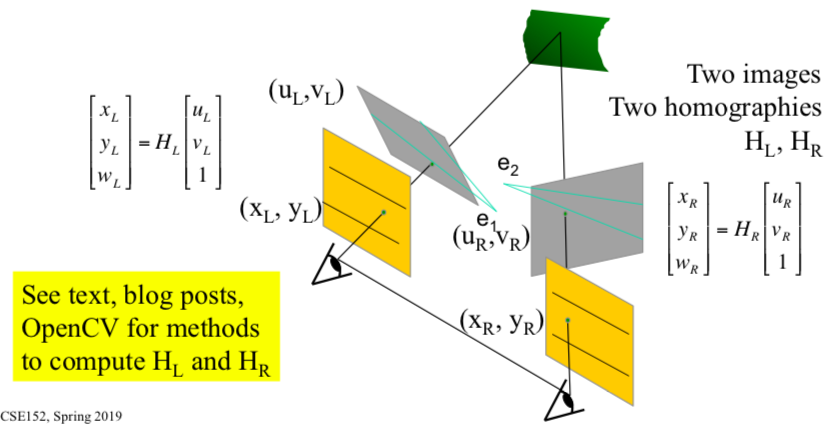
\includegraphics{image_rectification.png}

In this part you first need to complete the function compute\_epipole.
The function compute\_epipole is used to calculate the epipoles for a
given fundamental matrix and corner point correspondences in the two
images.

Using the compute\_epipoles function and the given
compute\_matching\_homographies function, we get \(H_L\) and \(H_R\).
Then we can complete the function image\_rectification to find the
rectified images and plot the parallel epipolar lines using the
plot\_epipolar\_lines function from above. You need to run this for both
the matrix and the warrior images. A sample output is provided below:
\includegraphics{sample_rectification.png}

    \subsubsection{Compute Epipole {[}5 pts{]}}\label{compute-epipole-5-pts}

    \begin{Verbatim}[commandchars=\\\{\}]
{\color{incolor}In [{\color{incolor}41}]:} \PY{k}{def} \PY{n+nf}{compute\PYZus{}epipole}\PY{p}{(}\PY{n}{F}\PY{p}{)}\PY{p}{:}
             \PY{l+s+sd}{\PYZsq{}\PYZsq{}\PYZsq{}}
         \PY{l+s+sd}{    This function computes the epipoles for a given fundamental matrix and corner point correspondences}
         \PY{l+s+sd}{    input:}
         \PY{l+s+sd}{    F\PYZhy{}\PYZhy{}\PYZgt{} Fundamental matrix}
         \PY{l+s+sd}{    output:}
         \PY{l+s+sd}{    e1\PYZhy{}\PYZhy{}\PYZgt{} corresponding epipole in image 1}
         \PY{l+s+sd}{    e2\PYZhy{}\PYZhy{}\PYZgt{} epipole in image2}
         \PY{l+s+sd}{    \PYZsq{}\PYZsq{}\PYZsq{}}
             \PY{l+s+sd}{\PYZdq{}\PYZdq{}\PYZdq{}}
         \PY{l+s+sd}{    Your Code Here!!!}
         \PY{l+s+sd}{    \PYZdq{}\PYZdq{}\PYZdq{}}
             
             \PY{n}{U}\PY{p}{,}\PY{n}{sigma}\PY{p}{,}\PY{n}{V} \PY{o}{=} \PY{n}{np}\PY{o}{.}\PY{n}{linalg}\PY{o}{.}\PY{n}{svd}\PY{p}{(}\PY{n}{F}\PY{p}{)}
             \PY{n}{e2} \PY{o}{=} \PY{n}{V}\PY{p}{[}\PY{o}{\PYZhy{}}\PY{l+m+mi}{1}\PY{p}{]}
         
             \PY{n}{U1}\PY{p}{,}\PY{n}{sigma1}\PY{p}{,}\PY{n}{V1} \PY{o}{=} \PY{n}{np}\PY{o}{.}\PY{n}{linalg}\PY{o}{.}\PY{n}{svd}\PY{p}{(}\PY{n}{np}\PY{o}{.}\PY{n}{array}\PY{p}{(}\PY{n}{F}\PY{p}{)}\PY{o}{.}\PY{n}{T}\PY{o}{.}\PY{n}{tolist}\PY{p}{(}\PY{p}{)}\PY{p}{)}
             \PY{n}{e1} \PY{o}{=} \PY{n}{V1}\PY{p}{[}\PY{o}{\PYZhy{}}\PY{l+m+mi}{1}\PY{p}{]}
             
             \PY{k}{return} \PY{n}{e1}\PY{o}{/}\PY{n}{e1}\PY{p}{[}\PY{l+m+mi}{2}\PY{p}{]}\PY{p}{,} \PY{n}{e2}\PY{o}{/}\PY{n}{e2}\PY{p}{[}\PY{l+m+mi}{2}\PY{p}{]}
\end{Verbatim}


    \subsubsection{Image Rectification {[}5
pts{]}}\label{image-rectification-5-pts}

    \begin{Verbatim}[commandchars=\\\{\}]
{\color{incolor}In [{\color{incolor}173}]:} \PY{k+kn}{import} \PY{n+nn}{math}
          \PY{k}{def} \PY{n+nf}{compute\PYZus{}matching\PYZus{}homographies}\PY{p}{(}\PY{n}{e2}\PY{p}{,} \PY{n}{F}\PY{p}{,} \PY{n}{im2}\PY{p}{,} \PY{n}{points1}\PY{p}{,} \PY{n}{points2}\PY{p}{)}\PY{p}{:}
              
              \PY{l+s+sd}{\PYZsq{}\PYZsq{}\PYZsq{}This function computes the homographies to get the rectified images}
          \PY{l+s+sd}{    input:}
          \PY{l+s+sd}{    e2\PYZhy{}\PYZhy{}\PYZgt{} epipole in image 2}
          \PY{l+s+sd}{    F\PYZhy{}\PYZhy{}\PYZgt{} the Fundamental matrix}
          \PY{l+s+sd}{    im2\PYZhy{}\PYZhy{}\PYZgt{} image2}
          \PY{l+s+sd}{    points1 \PYZhy{}\PYZhy{}\PYZgt{} corner points in image1}
          \PY{l+s+sd}{    points2\PYZhy{}\PYZhy{}\PYZgt{} corresponding corner points in image2}
          \PY{l+s+sd}{    output:}
          \PY{l+s+sd}{    H1\PYZhy{}\PYZhy{}\PYZgt{} Homography for image 1}
          \PY{l+s+sd}{    H2\PYZhy{}\PYZhy{}\PYZgt{} Homography for image 2}
          \PY{l+s+sd}{    \PYZsq{}\PYZsq{}\PYZsq{}}
              \PY{c+c1}{\PYZsh{} calculate H2}
              \PY{n}{width} \PY{o}{=} \PY{n}{im2}\PY{o}{.}\PY{n}{shape}\PY{p}{[}\PY{l+m+mi}{1}\PY{p}{]}
              \PY{n}{height} \PY{o}{=} \PY{n}{im2}\PY{o}{.}\PY{n}{shape}\PY{p}{[}\PY{l+m+mi}{0}\PY{p}{]}
          
              \PY{n}{T} \PY{o}{=} \PY{n}{np}\PY{o}{.}\PY{n}{identity}\PY{p}{(}\PY{l+m+mi}{3}\PY{p}{)}
              \PY{n}{T}\PY{p}{[}\PY{l+m+mi}{0}\PY{p}{]}\PY{p}{[}\PY{l+m+mi}{2}\PY{p}{]} \PY{o}{=} \PY{o}{\PYZhy{}}\PY{l+m+mf}{1.0} \PY{o}{*} \PY{n}{width} \PY{o}{/} \PY{l+m+mi}{2}
              \PY{n}{T}\PY{p}{[}\PY{l+m+mi}{1}\PY{p}{]}\PY{p}{[}\PY{l+m+mi}{2}\PY{p}{]} \PY{o}{=} \PY{o}{\PYZhy{}}\PY{l+m+mf}{1.0} \PY{o}{*} \PY{n}{height} \PY{o}{/} \PY{l+m+mi}{2}
          
              \PY{n}{e} \PY{o}{=} \PY{n}{T}\PY{o}{.}\PY{n}{dot}\PY{p}{(}\PY{n}{e2}\PY{p}{)}
              \PY{n}{e1\PYZus{}prime} \PY{o}{=} \PY{n}{e}\PY{p}{[}\PY{l+m+mi}{0}\PY{p}{]}
              \PY{n}{e2\PYZus{}prime} \PY{o}{=} \PY{n}{e}\PY{p}{[}\PY{l+m+mi}{1}\PY{p}{]}
              \PY{k}{if} \PY{n}{e1\PYZus{}prime} \PY{o}{\PYZgt{}}\PY{o}{=} \PY{l+m+mi}{0}\PY{p}{:}
                  \PY{n}{alpha} \PY{o}{=} \PY{l+m+mf}{1.0}
              \PY{k}{else}\PY{p}{:}
                  \PY{n}{alpha} \PY{o}{=} \PY{o}{\PYZhy{}}\PY{l+m+mf}{1.0}
          
              \PY{n}{R} \PY{o}{=} \PY{n}{np}\PY{o}{.}\PY{n}{identity}\PY{p}{(}\PY{l+m+mi}{3}\PY{p}{)}
              \PY{n}{R}\PY{p}{[}\PY{l+m+mi}{0}\PY{p}{]}\PY{p}{[}\PY{l+m+mi}{0}\PY{p}{]} \PY{o}{=} \PY{n}{alpha} \PY{o}{*} \PY{n}{e1\PYZus{}prime} \PY{o}{/} \PY{n}{np}\PY{o}{.}\PY{n}{sqrt}\PY{p}{(}\PY{n}{e1\PYZus{}prime}\PY{o}{*}\PY{o}{*}\PY{l+m+mi}{2} \PY{o}{+} \PY{n}{e2\PYZus{}prime}\PY{o}{*}\PY{o}{*}\PY{l+m+mi}{2}\PY{p}{)}
              \PY{n}{R}\PY{p}{[}\PY{l+m+mi}{0}\PY{p}{]}\PY{p}{[}\PY{l+m+mi}{1}\PY{p}{]} \PY{o}{=} \PY{n}{alpha} \PY{o}{*} \PY{n}{e2\PYZus{}prime} \PY{o}{/} \PY{n}{np}\PY{o}{.}\PY{n}{sqrt}\PY{p}{(}\PY{n}{e1\PYZus{}prime}\PY{o}{*}\PY{o}{*}\PY{l+m+mi}{2} \PY{o}{+} \PY{n}{e2\PYZus{}prime}\PY{o}{*}\PY{o}{*}\PY{l+m+mi}{2}\PY{p}{)}
              \PY{n}{R}\PY{p}{[}\PY{l+m+mi}{1}\PY{p}{]}\PY{p}{[}\PY{l+m+mi}{0}\PY{p}{]} \PY{o}{=} \PY{o}{\PYZhy{}} \PY{n}{alpha} \PY{o}{*} \PY{n}{e2\PYZus{}prime} \PY{o}{/} \PY{n}{np}\PY{o}{.}\PY{n}{sqrt}\PY{p}{(}\PY{n}{e1\PYZus{}prime}\PY{o}{*}\PY{o}{*}\PY{l+m+mi}{2} \PY{o}{+} \PY{n}{e2\PYZus{}prime}\PY{o}{*}\PY{o}{*}\PY{l+m+mi}{2}\PY{p}{)}
              \PY{n}{R}\PY{p}{[}\PY{l+m+mi}{1}\PY{p}{]}\PY{p}{[}\PY{l+m+mi}{1}\PY{p}{]} \PY{o}{=} \PY{n}{alpha} \PY{o}{*} \PY{n}{e1\PYZus{}prime} \PY{o}{/} \PY{n}{np}\PY{o}{.}\PY{n}{sqrt}\PY{p}{(}\PY{n}{e1\PYZus{}prime}\PY{o}{*}\PY{o}{*}\PY{l+m+mi}{2} \PY{o}{+} \PY{n}{e2\PYZus{}prime}\PY{o}{*}\PY{o}{*}\PY{l+m+mi}{2}\PY{p}{)}
          
              \PY{n}{f} \PY{o}{=} \PY{n}{R}\PY{o}{.}\PY{n}{dot}\PY{p}{(}\PY{n}{e}\PY{p}{)}\PY{p}{[}\PY{l+m+mi}{0}\PY{p}{]}
              \PY{n}{G} \PY{o}{=} \PY{n}{np}\PY{o}{.}\PY{n}{identity}\PY{p}{(}\PY{l+m+mi}{3}\PY{p}{)}
              \PY{n}{G}\PY{p}{[}\PY{l+m+mi}{2}\PY{p}{]}\PY{p}{[}\PY{l+m+mi}{0}\PY{p}{]} \PY{o}{=} \PY{o}{\PYZhy{}} \PY{l+m+mf}{1.0} \PY{o}{/} \PY{n}{f}
          
              \PY{n}{H2} \PY{o}{=} \PY{n}{np}\PY{o}{.}\PY{n}{linalg}\PY{o}{.}\PY{n}{inv}\PY{p}{(}\PY{n}{T}\PY{p}{)}\PY{o}{.}\PY{n}{dot}\PY{p}{(}\PY{n}{G}\PY{o}{.}\PY{n}{dot}\PY{p}{(}\PY{n}{R}\PY{o}{.}\PY{n}{dot}\PY{p}{(}\PY{n}{T}\PY{p}{)}\PY{p}{)}\PY{p}{)}
          
              \PY{c+c1}{\PYZsh{} calculate H1}
              \PY{n}{e\PYZus{}prime} \PY{o}{=} \PY{n}{np}\PY{o}{.}\PY{n}{zeros}\PY{p}{(}\PY{p}{(}\PY{l+m+mi}{3}\PY{p}{,} \PY{l+m+mi}{3}\PY{p}{)}\PY{p}{)}
              \PY{n}{e\PYZus{}prime}\PY{p}{[}\PY{l+m+mi}{0}\PY{p}{]}\PY{p}{[}\PY{l+m+mi}{1}\PY{p}{]} \PY{o}{=} \PY{o}{\PYZhy{}}\PY{n}{e2}\PY{p}{[}\PY{l+m+mi}{2}\PY{p}{]}
              \PY{n}{e\PYZus{}prime}\PY{p}{[}\PY{l+m+mi}{0}\PY{p}{]}\PY{p}{[}\PY{l+m+mi}{2}\PY{p}{]} \PY{o}{=} \PY{n}{e2}\PY{p}{[}\PY{l+m+mi}{1}\PY{p}{]}
              \PY{n}{e\PYZus{}prime}\PY{p}{[}\PY{l+m+mi}{1}\PY{p}{]}\PY{p}{[}\PY{l+m+mi}{0}\PY{p}{]} \PY{o}{=} \PY{n}{e2}\PY{p}{[}\PY{l+m+mi}{2}\PY{p}{]}
              \PY{n}{e\PYZus{}prime}\PY{p}{[}\PY{l+m+mi}{1}\PY{p}{]}\PY{p}{[}\PY{l+m+mi}{2}\PY{p}{]} \PY{o}{=} \PY{o}{\PYZhy{}}\PY{n}{e2}\PY{p}{[}\PY{l+m+mi}{0}\PY{p}{]}
              \PY{n}{e\PYZus{}prime}\PY{p}{[}\PY{l+m+mi}{2}\PY{p}{]}\PY{p}{[}\PY{l+m+mi}{0}\PY{p}{]} \PY{o}{=} \PY{o}{\PYZhy{}}\PY{n}{e2}\PY{p}{[}\PY{l+m+mi}{1}\PY{p}{]}
              \PY{n}{e\PYZus{}prime}\PY{p}{[}\PY{l+m+mi}{2}\PY{p}{]}\PY{p}{[}\PY{l+m+mi}{1}\PY{p}{]} \PY{o}{=} \PY{n}{e2}\PY{p}{[}\PY{l+m+mi}{0}\PY{p}{]}
          
              \PY{n}{v} \PY{o}{=} \PY{n}{np}\PY{o}{.}\PY{n}{array}\PY{p}{(}\PY{p}{[}\PY{l+m+mi}{1}\PY{p}{,} \PY{l+m+mi}{1}\PY{p}{,} \PY{l+m+mi}{1}\PY{p}{]}\PY{p}{)}
              \PY{n}{M} \PY{o}{=} \PY{n}{e\PYZus{}prime}\PY{o}{.}\PY{n}{dot}\PY{p}{(}\PY{n}{F}\PY{p}{)} \PY{o}{+} \PY{n}{np}\PY{o}{.}\PY{n}{outer}\PY{p}{(}\PY{n}{e2}\PY{p}{,} \PY{n}{v}\PY{p}{)}
          
              \PY{n}{points1\PYZus{}hat} \PY{o}{=} \PY{n}{H2}\PY{o}{.}\PY{n}{dot}\PY{p}{(}\PY{n}{M}\PY{o}{.}\PY{n}{dot}\PY{p}{(}\PY{n}{points1}\PY{o}{.}\PY{n}{T}\PY{p}{)}\PY{p}{)}\PY{o}{.}\PY{n}{T}
              \PY{n}{points2\PYZus{}hat} \PY{o}{=} \PY{n}{H2}\PY{o}{.}\PY{n}{dot}\PY{p}{(}\PY{n}{points2}\PY{o}{.}\PY{n}{T}\PY{p}{)}\PY{o}{.}\PY{n}{T}
          
              \PY{n}{W} \PY{o}{=} \PY{n}{points1\PYZus{}hat} \PY{o}{/} \PY{n}{points1\PYZus{}hat}\PY{p}{[}\PY{p}{:}\PY{p}{,} \PY{l+m+mi}{2}\PY{p}{]}\PY{o}{.}\PY{n}{reshape}\PY{p}{(}\PY{o}{\PYZhy{}}\PY{l+m+mi}{1}\PY{p}{,} \PY{l+m+mi}{1}\PY{p}{)}
              \PY{n}{b} \PY{o}{=} \PY{p}{(}\PY{n}{points2\PYZus{}hat} \PY{o}{/} \PY{n}{points2\PYZus{}hat}\PY{p}{[}\PY{p}{:}\PY{p}{,} \PY{l+m+mi}{2}\PY{p}{]}\PY{o}{.}\PY{n}{reshape}\PY{p}{(}\PY{o}{\PYZhy{}}\PY{l+m+mi}{1}\PY{p}{,} \PY{l+m+mi}{1}\PY{p}{)}\PY{p}{)}\PY{p}{[}\PY{p}{:}\PY{p}{,} \PY{l+m+mi}{0}\PY{p}{]}
          
              \PY{c+c1}{\PYZsh{} least square problem}
              \PY{n}{a1}\PY{p}{,} \PY{n}{a2}\PY{p}{,} \PY{n}{a3} \PY{o}{=} \PY{n}{np}\PY{o}{.}\PY{n}{linalg}\PY{o}{.}\PY{n}{lstsq}\PY{p}{(}\PY{n}{W}\PY{p}{,} \PY{n}{b}\PY{p}{)}\PY{p}{[}\PY{l+m+mi}{0}\PY{p}{]}
              \PY{n}{HA} \PY{o}{=} \PY{n}{np}\PY{o}{.}\PY{n}{identity}\PY{p}{(}\PY{l+m+mi}{3}\PY{p}{)}
              \PY{n}{HA}\PY{p}{[}\PY{l+m+mi}{0}\PY{p}{]} \PY{o}{=} \PY{n}{np}\PY{o}{.}\PY{n}{array}\PY{p}{(}\PY{p}{[}\PY{n}{a1}\PY{p}{,} \PY{n}{a2}\PY{p}{,} \PY{n}{a3}\PY{p}{]}\PY{p}{)}
          
              \PY{n}{H1} \PY{o}{=} \PY{n}{HA}\PY{o}{.}\PY{n}{dot}\PY{p}{(}\PY{n}{H2}\PY{p}{)}\PY{o}{.}\PY{n}{dot}\PY{p}{(}\PY{n}{M}\PY{p}{)}
              \PY{k}{return} \PY{n}{H1}\PY{p}{,} \PY{n}{H2}
          
          \PY{k}{def} \PY{n+nf}{image\PYZus{}rectification}\PY{p}{(}\PY{n}{im1}\PY{p}{,}\PY{n}{im2}\PY{p}{,}\PY{n}{points1}\PY{p}{,}\PY{n}{points2}\PY{p}{)}\PY{p}{:}
              \PY{l+s+sd}{\PYZsq{}\PYZsq{}\PYZsq{}This function provides the rectified images along with the new corner points as outputs for a given pair of }
          \PY{l+s+sd}{    images with corner correspondences}
          \PY{l+s+sd}{    input:}
          \PY{l+s+sd}{    im1\PYZhy{}\PYZhy{}\PYZgt{} image1}
          \PY{l+s+sd}{    im2\PYZhy{}\PYZhy{}\PYZgt{} image2}
          \PY{l+s+sd}{    points1\PYZhy{}\PYZhy{}\PYZgt{} corner points in image1}
          \PY{l+s+sd}{    points2\PYZhy{}\PYZhy{}\PYZgt{} corner points in image2}
          \PY{l+s+sd}{    output:}
          \PY{l+s+sd}{    rectified\PYZus{}im1\PYZhy{}\PYZhy{}\PYZgt{}rectified image 1}
          \PY{l+s+sd}{    rectified\PYZus{}im2\PYZhy{}\PYZhy{}\PYZgt{}rectified image 2}
          \PY{l+s+sd}{    new\PYZus{}cor1\PYZhy{}\PYZhy{}\PYZgt{} new corners in the rectified image 1}
          \PY{l+s+sd}{    new\PYZus{}cor2\PYZhy{}\PYZhy{}\PYZgt{} new corners in the rectified image 2}
          \PY{l+s+sd}{    \PYZsq{}\PYZsq{}\PYZsq{}}
              
              \PY{l+s+sd}{\PYZsq{}\PYZsq{}\PYZsq{}}
          \PY{l+s+sd}{    Your Code Here!!!}
          \PY{l+s+sd}{    \PYZsq{}\PYZsq{}\PYZsq{}}
              \PY{n}{F} \PY{o}{=} \PY{n}{fundamental\PYZus{}matrix}\PY{p}{(}\PY{n}{points1}\PY{p}{,} \PY{n}{points2}\PY{p}{)}
              \PY{n}{e1}\PY{p}{,} \PY{n}{e2} \PY{o}{=} \PY{n}{compute\PYZus{}epipole}\PY{p}{(}\PY{n}{F}\PY{p}{)}
              \PY{n}{height}\PY{p}{,} \PY{n}{width} \PY{o}{=} \PY{n}{im1}\PY{o}{.}\PY{n}{shape}
              \PY{n}{H1}\PY{p}{,} \PY{n}{H2} \PY{o}{=} \PY{n}{compute\PYZus{}matching\PYZus{}homographies}\PY{p}{(}\PY{n}{e2}\PY{p}{,} \PY{n}{F}\PY{o}{.}\PY{n}{T}\PY{p}{,} \PY{n}{im2}\PY{p}{,} \PY{n}{points1}\PY{o}{.}\PY{n}{T}\PY{p}{,} \PY{n}{points2}\PY{o}{.}\PY{n}{T}\PY{p}{)}
              \PY{n}{H1\PYZus{}I} \PY{o}{=} \PY{n}{np}\PY{o}{.}\PY{n}{linalg}\PY{o}{.}\PY{n}{inv}\PY{p}{(}\PY{n}{H1}\PY{p}{)}
              \PY{n}{H2\PYZus{}I} \PY{o}{=} \PY{n}{np}\PY{o}{.}\PY{n}{linalg}\PY{o}{.}\PY{n}{inv}\PY{p}{(}\PY{n}{H2}\PY{p}{)}
              
              
              \PY{c+c1}{\PYZsh{} Calculate the output coordinates}
              \PY{n}{points\PYZus{}1} \PY{o}{=} \PY{n}{H1}\PY{o}{.}\PY{n}{dot}\PY{p}{(}\PY{n}{points1}\PY{p}{)}
              \PY{n}{points\PYZus{}2} \PY{o}{=} \PY{n}{H2}\PY{o}{.}\PY{n}{dot}\PY{p}{(}\PY{n}{points2}\PY{p}{)}
              \PY{c+c1}{\PYZsh{}points\PYZus{}1 = from\PYZus{}homog(points\PYZus{}1)}
              \PY{c+c1}{\PYZsh{}points\PYZus{}2 = from\PYZus{}homog(points\PYZus{}2)}
              
              \PY{n}{orig\PYZus{}cors} \PY{o}{=} \PY{p}{[}\PY{p}{[}\PY{l+m+mi}{0}\PY{p}{,}\PY{l+m+mi}{0}\PY{p}{,}\PY{n}{width}\PY{p}{,} \PY{n}{width}\PY{p}{]}\PY{p}{,} \PY{p}{[}\PY{l+m+mi}{0}\PY{p}{,}\PY{n}{height}\PY{p}{,}\PY{l+m+mi}{0}\PY{p}{,} \PY{n}{height}\PY{p}{]}\PY{p}{,} \PY{p}{[}\PY{l+m+mi}{1}\PY{p}{,}\PY{l+m+mi}{1}\PY{p}{,}\PY{l+m+mi}{1}\PY{p}{,}\PY{l+m+mi}{1}\PY{p}{]}\PY{p}{]}
              \PY{n}{new\PYZus{}cors1} \PY{o}{=} \PY{n}{H1}\PY{o}{.}\PY{n}{dot}\PY{p}{(}\PY{n}{orig\PYZus{}cors}\PY{p}{)}
              \PY{n}{new\PYZus{}cors2} \PY{o}{=} \PY{n}{H2}\PY{o}{.}\PY{n}{dot}\PY{p}{(}\PY{n}{orig\PYZus{}cors}\PY{p}{)}
              \PY{n}{new\PYZus{}cors1} \PY{o}{=} \PY{n}{from\PYZus{}homog}\PY{p}{(}\PY{n}{new\PYZus{}cors1}\PY{p}{)}
              \PY{n}{new\PYZus{}cors2} \PY{o}{=} \PY{n}{from\PYZus{}homog}\PY{p}{(}\PY{n}{new\PYZus{}cors2}\PY{p}{)}
              
              \PY{c+c1}{\PYZsh{}print(new\PYZus{}cors1)}
              \PY{c+c1}{\PYZsh{}print(new\PYZus{}cors2)}
              
              \PY{n}{right1} \PY{o}{=} \PY{n}{math}\PY{o}{.}\PY{n}{ceil}\PY{p}{(}\PY{n+nb}{max}\PY{p}{(}\PY{n}{new\PYZus{}cors1}\PY{p}{[}\PY{l+m+mi}{0}\PY{p}{]}\PY{p}{)}\PY{p}{)}
              \PY{n}{left1} \PY{o}{=} \PY{n}{math}\PY{o}{.}\PY{n}{floor}\PY{p}{(}\PY{n+nb}{min}\PY{p}{(}\PY{n}{new\PYZus{}cors1}\PY{p}{[}\PY{l+m+mi}{0}\PY{p}{]}\PY{p}{)}\PY{p}{)}
              \PY{n}{top1} \PY{o}{=} \PY{n}{math}\PY{o}{.}\PY{n}{floor}\PY{p}{(}\PY{n+nb}{min}\PY{p}{(}\PY{n}{new\PYZus{}cors1}\PY{p}{[}\PY{l+m+mi}{1}\PY{p}{]}\PY{p}{)}\PY{p}{)}
              \PY{n}{bot1} \PY{o}{=} \PY{n}{math}\PY{o}{.}\PY{n}{ceil}\PY{p}{(}\PY{n+nb}{max}\PY{p}{(}\PY{n}{new\PYZus{}cors1}\PY{p}{[}\PY{l+m+mi}{1}\PY{p}{]}\PY{p}{)}\PY{p}{)}
              
              \PY{n}{x1} \PY{o}{=} \PY{n}{np}\PY{o}{.}\PY{n}{arange}\PY{p}{(}\PY{n}{left1}\PY{p}{,} \PY{n}{right1}\PY{p}{)}
              \PY{n}{y1} \PY{o}{=} \PY{n}{np}\PY{o}{.}\PY{n}{arange}\PY{p}{(}\PY{n}{top1}\PY{p}{,} \PY{n}{bot1}\PY{p}{)}
              \PY{n}{xx1}\PY{p}{,} \PY{n}{yy1} \PY{o}{=} \PY{n}{np}\PY{o}{.}\PY{n}{meshgrid}\PY{p}{(}\PY{n}{x1}\PY{p}{,} \PY{n}{y1}\PY{p}{)}
              \PY{n}{xycord\PYZus{}old1} \PY{o}{=} \PY{n}{np}\PY{o}{.}\PY{n}{stack}\PY{p}{(}\PY{p}{(}\PY{n}{xx1}\PY{p}{,}\PY{n}{yy1}\PY{p}{)}\PY{p}{,} \PY{n}{axis}\PY{o}{=} \PY{l+m+mi}{0}\PY{p}{)}\PY{o}{.}\PY{n}{reshape}\PY{p}{(}\PY{l+m+mi}{2}\PY{p}{,} \PY{o}{\PYZhy{}}\PY{l+m+mi}{1}\PY{p}{)}
              
              \PY{n}{xycord1} \PY{o}{=} \PY{n}{to\PYZus{}homog}\PY{p}{(}\PY{n}{xycord\PYZus{}old1}\PY{p}{)}
              \PY{n}{xycord1} \PY{o}{=} \PY{n}{H1\PYZus{}I}\PY{o}{.}\PY{n}{dot}\PY{p}{(}\PY{n}{xycord1}\PY{p}{)}
              \PY{n}{xycord1} \PY{o}{=} \PY{n}{from\PYZus{}homog}\PY{p}{(}\PY{n}{xycord1}\PY{p}{)}
              
              \PY{n}{rectified\PYZus{}im1} \PY{o}{=} \PY{n}{np}\PY{o}{.}\PY{n}{zeros}\PY{p}{(}\PY{p}{(}\PY{n}{bot1}\PY{o}{\PYZhy{}} \PY{n}{top1}\PY{p}{,} \PY{n}{right1}\PY{o}{\PYZhy{}} \PY{n}{left1}\PY{p}{)}\PY{p}{)}
              \PY{k}{for} \PY{n}{i} \PY{o+ow}{in} \PY{n+nb}{range}\PY{p}{(}\PY{n+nb}{len}\PY{p}{(}\PY{n}{xycord1}\PY{p}{[}\PY{l+m+mi}{0}\PY{p}{]}\PY{p}{)}\PY{p}{)}\PY{p}{:}
                  \PY{n}{new}  \PY{o}{=} \PY{n}{xycord\PYZus{}old1}\PY{p}{[}\PY{p}{:}\PY{p}{,} \PY{n}{i}\PY{p}{:}\PY{n}{i}\PY{o}{+}\PY{l+m+mi}{1}\PY{p}{]}
                  \PY{n}{new}  \PY{o}{=} \PY{p}{[}\PY{n}{new}\PY{p}{[}\PY{l+m+mi}{0}\PY{p}{]}\PY{p}{[}\PY{l+m+mi}{0}\PY{p}{]}\PY{p}{,} \PY{n}{new}\PY{p}{[}\PY{l+m+mi}{1}\PY{p}{]}\PY{p}{[}\PY{l+m+mi}{0}\PY{p}{]}\PY{p}{]}
                  \PY{n}{orig} \PY{o}{=} \PY{n}{xycord1}\PY{p}{[}\PY{p}{:}\PY{p}{,} \PY{n}{i}\PY{p}{:}\PY{n}{i}\PY{o}{+}\PY{l+m+mi}{1}\PY{p}{]}
                  \PY{n}{orig} \PY{o}{=} \PY{p}{[}\PY{n}{math}\PY{o}{.}\PY{n}{floor}\PY{p}{(}\PY{n}{orig}\PY{p}{[}\PY{l+m+mi}{0}\PY{p}{]}\PY{p}{[}\PY{l+m+mi}{0}\PY{p}{]}\PY{p}{)}\PY{p}{,} \PY{n}{math}\PY{o}{.}\PY{n}{floor}\PY{p}{(}\PY{n}{orig}\PY{p}{[}\PY{l+m+mi}{1}\PY{p}{]}\PY{p}{[}\PY{l+m+mi}{0}\PY{p}{]}\PY{p}{)}\PY{p}{]}
                  \PY{c+c1}{\PYZsh{}print(new)}
                  \PY{c+c1}{\PYZsh{}print(orig)}
                  \PY{k}{if} \PY{n}{orig}\PY{p}{[}\PY{l+m+mi}{0}\PY{p}{]} \PY{o}{\PYZgt{}}\PY{o}{=} \PY{l+m+mi}{0} \PY{o+ow}{and} \PY{n}{orig}\PY{p}{[}\PY{l+m+mi}{0}\PY{p}{]} \PY{o}{\PYZlt{}} \PY{n}{width} \PY{o+ow}{and} \PY{n}{orig}\PY{p}{[}\PY{l+m+mi}{1}\PY{p}{]} \PY{o}{\PYZgt{}}\PY{o}{=} \PY{l+m+mi}{0} \PY{o+ow}{and} \PY{n}{orig}\PY{p}{[}\PY{l+m+mi}{1}\PY{p}{]} \PY{o}{\PYZlt{}} \PY{n}{height}\PY{p}{:}
                      \PY{n}{rectified\PYZus{}im1}\PY{p}{[}\PY{n}{new}\PY{p}{[}\PY{l+m+mi}{1}\PY{p}{]} \PY{o}{\PYZhy{}} \PY{n}{top1}\PY{p}{]}\PY{p}{[}\PY{n}{new}\PY{p}{[}\PY{l+m+mi}{0}\PY{p}{]}\PY{o}{\PYZhy{}}\PY{n}{left1}\PY{p}{]} \PY{o}{=} \PY{n}{im1}\PY{p}{[}\PY{n}{orig}\PY{p}{[}\PY{l+m+mi}{1}\PY{p}{]}\PY{p}{]}\PY{p}{[}\PY{n}{orig}\PY{p}{[}\PY{l+m+mi}{0}\PY{p}{]}\PY{p}{]}
              
              
              
              
              \PY{n}{right2} \PY{o}{=} \PY{n}{math}\PY{o}{.}\PY{n}{ceil}\PY{p}{(}\PY{n+nb}{max}\PY{p}{(}\PY{n}{new\PYZus{}cors2}\PY{p}{[}\PY{l+m+mi}{0}\PY{p}{]}\PY{p}{)}\PY{p}{)}
              \PY{n}{left2} \PY{o}{=} \PY{n}{math}\PY{o}{.}\PY{n}{floor}\PY{p}{(}\PY{n+nb}{min}\PY{p}{(}\PY{n}{new\PYZus{}cors2}\PY{p}{[}\PY{l+m+mi}{0}\PY{p}{]}\PY{p}{)}\PY{p}{)}
              \PY{n}{top2} \PY{o}{=} \PY{n}{math}\PY{o}{.}\PY{n}{floor}\PY{p}{(}\PY{n+nb}{min}\PY{p}{(}\PY{n}{new\PYZus{}cors2}\PY{p}{[}\PY{l+m+mi}{1}\PY{p}{]}\PY{p}{)}\PY{p}{)}
              \PY{n}{bot2} \PY{o}{=} \PY{n}{math}\PY{o}{.}\PY{n}{ceil}\PY{p}{(}\PY{n+nb}{max}\PY{p}{(}\PY{n}{new\PYZus{}cors2}\PY{p}{[}\PY{l+m+mi}{1}\PY{p}{]}\PY{p}{)}\PY{p}{)}    
              
              \PY{n}{x2} \PY{o}{=} \PY{n}{np}\PY{o}{.}\PY{n}{arange}\PY{p}{(}\PY{n}{left2}\PY{p}{,} \PY{n}{right2}\PY{p}{)}
              \PY{n}{y2} \PY{o}{=} \PY{n}{np}\PY{o}{.}\PY{n}{arange}\PY{p}{(}\PY{n}{top2}\PY{p}{,} \PY{n}{bot2}\PY{p}{)}
              \PY{n}{xx2}\PY{p}{,} \PY{n}{yy2} \PY{o}{=} \PY{n}{np}\PY{o}{.}\PY{n}{meshgrid}\PY{p}{(}\PY{n}{x2}\PY{p}{,} \PY{n}{y2}\PY{p}{)}
              \PY{n}{xycord\PYZus{}old2} \PY{o}{=} \PY{n}{np}\PY{o}{.}\PY{n}{stack}\PY{p}{(}\PY{p}{(}\PY{n}{xx2}\PY{p}{,}\PY{n}{yy2}\PY{p}{)}\PY{p}{,} \PY{n}{axis}\PY{o}{=} \PY{l+m+mi}{0}\PY{p}{)}\PY{o}{.}\PY{n}{reshape}\PY{p}{(}\PY{l+m+mi}{2}\PY{p}{,} \PY{o}{\PYZhy{}}\PY{l+m+mi}{1}\PY{p}{)}
             
              \PY{n}{xycord2} \PY{o}{=} \PY{n}{to\PYZus{}homog}\PY{p}{(}\PY{n}{xycord\PYZus{}old2}\PY{p}{)}
              \PY{n}{xycord2} \PY{o}{=} \PY{n}{H2\PYZus{}I}\PY{o}{.}\PY{n}{dot}\PY{p}{(}\PY{n}{xycord2}\PY{p}{)}
              \PY{n}{xycord2} \PY{o}{=} \PY{n}{from\PYZus{}homog}\PY{p}{(}\PY{n}{xycord2}\PY{p}{)}
              
              \PY{n}{rectified\PYZus{}im2} \PY{o}{=} \PY{n}{np}\PY{o}{.}\PY{n}{zeros}\PY{p}{(}\PY{p}{(}\PY{n}{bot2} \PY{o}{\PYZhy{}} \PY{n}{top2}\PY{p}{,} \PY{n}{right2} \PY{o}{\PYZhy{}} \PY{n}{left2}\PY{p}{)}\PY{p}{)}
              \PY{k}{for} \PY{n}{i} \PY{o+ow}{in} \PY{n+nb}{range}\PY{p}{(}\PY{n+nb}{len}\PY{p}{(}\PY{n}{xycord2}\PY{p}{[}\PY{l+m+mi}{0}\PY{p}{]}\PY{p}{)}\PY{p}{)}\PY{p}{:}
                  \PY{n}{new}  \PY{o}{=} \PY{n}{xycord\PYZus{}old2}\PY{p}{[}\PY{p}{:}\PY{p}{,} \PY{n}{i}\PY{p}{:}\PY{n}{i}\PY{o}{+}\PY{l+m+mi}{1}\PY{p}{]}
                  \PY{n}{new}  \PY{o}{=} \PY{p}{[}\PY{n}{new}\PY{p}{[}\PY{l+m+mi}{0}\PY{p}{]}\PY{p}{[}\PY{l+m+mi}{0}\PY{p}{]}\PY{p}{,} \PY{n}{new}\PY{p}{[}\PY{l+m+mi}{1}\PY{p}{]}\PY{p}{[}\PY{l+m+mi}{0}\PY{p}{]}\PY{p}{]}
                  \PY{n}{orig} \PY{o}{=} \PY{n}{xycord2}\PY{p}{[}\PY{p}{:}\PY{p}{,} \PY{n}{i}\PY{p}{:}\PY{n}{i}\PY{o}{+}\PY{l+m+mi}{1}\PY{p}{]}
                  \PY{n}{orig} \PY{o}{=} \PY{p}{[}\PY{n}{math}\PY{o}{.}\PY{n}{floor}\PY{p}{(}\PY{n}{orig}\PY{p}{[}\PY{l+m+mi}{0}\PY{p}{]}\PY{p}{[}\PY{l+m+mi}{0}\PY{p}{]}\PY{p}{)}\PY{p}{,} \PY{n}{math}\PY{o}{.}\PY{n}{floor}\PY{p}{(}\PY{n}{orig}\PY{p}{[}\PY{l+m+mi}{1}\PY{p}{]}\PY{p}{[}\PY{l+m+mi}{0}\PY{p}{]}\PY{p}{)}\PY{p}{]}
                  \PY{k}{if} \PY{n}{orig}\PY{p}{[}\PY{l+m+mi}{0}\PY{p}{]} \PY{o}{\PYZgt{}}\PY{o}{=} \PY{l+m+mi}{0} \PY{o+ow}{and} \PY{n}{orig}\PY{p}{[}\PY{l+m+mi}{0}\PY{p}{]} \PY{o}{\PYZlt{}} \PY{n}{width} \PY{o+ow}{and} \PY{n}{orig}\PY{p}{[}\PY{l+m+mi}{1}\PY{p}{]} \PY{o}{\PYZgt{}}\PY{o}{=} \PY{l+m+mi}{0} \PY{o+ow}{and} \PY{n}{orig}\PY{p}{[}\PY{l+m+mi}{1}\PY{p}{]} \PY{o}{\PYZlt{}} \PY{n}{height}\PY{p}{:}
                      \PY{n}{rectified\PYZus{}im2}\PY{p}{[}\PY{n}{new}\PY{p}{[}\PY{l+m+mi}{1}\PY{p}{]} \PY{o}{\PYZhy{}} \PY{n}{top2}\PY{p}{]}\PY{p}{[}\PY{n}{new}\PY{p}{[}\PY{l+m+mi}{0}\PY{p}{]}\PY{o}{\PYZhy{}}\PY{n}{left2}\PY{p}{]} \PY{o}{=} \PY{n}{im2}\PY{p}{[}\PY{n}{orig}\PY{p}{[}\PY{l+m+mi}{1}\PY{p}{]}\PY{p}{]}\PY{p}{[}\PY{n}{orig}\PY{p}{[}\PY{l+m+mi}{0}\PY{p}{]}\PY{p}{]}
              
              \PY{c+c1}{\PYZsh{} compute\PYZus{}matching\PYZus{}homographies(e2, F, im2, points1, points2)}
              \PY{c+c1}{\PYZsh{} compute\PYZus{}epipole(F)}
              
              \PY{n}{points\PYZus{}1} \PY{o}{=} \PY{n}{from\PYZus{}homog}\PY{p}{(}\PY{n}{points\PYZus{}1}\PY{p}{)}
              \PY{k}{for} \PY{n}{i} \PY{o+ow}{in} \PY{n+nb}{range}\PY{p}{(}\PY{n+nb}{len}\PY{p}{(}\PY{n}{points\PYZus{}1}\PY{p}{[}\PY{l+m+mi}{0}\PY{p}{]}\PY{p}{)}\PY{p}{)}\PY{p}{:}
                  \PY{n}{points\PYZus{}1}\PY{p}{[}\PY{l+m+mi}{1}\PY{p}{]}\PY{p}{[}\PY{n}{i}\PY{p}{]} \PY{o}{\PYZhy{}}\PY{o}{=} \PY{n}{top1}
                  \PY{n}{points\PYZus{}1}\PY{p}{[}\PY{l+m+mi}{0}\PY{p}{]}\PY{p}{[}\PY{n}{i}\PY{p}{]} \PY{o}{\PYZhy{}}\PY{o}{=} \PY{n}{left1}
              \PY{n}{points\PYZus{}1} \PY{o}{=} \PY{n}{to\PYZus{}homog}\PY{p}{(}\PY{n}{points\PYZus{}1}\PY{p}{)}    
              
              \PY{n}{points\PYZus{}2} \PY{o}{=} \PY{n}{from\PYZus{}homog}\PY{p}{(}\PY{n}{points\PYZus{}2}\PY{p}{)}
              \PY{k}{for} \PY{n}{j} \PY{o+ow}{in} \PY{n+nb}{range}\PY{p}{(}\PY{n+nb}{len}\PY{p}{(}\PY{n}{points\PYZus{}2}\PY{p}{[}\PY{l+m+mi}{0}\PY{p}{]}\PY{p}{)}\PY{p}{)}\PY{p}{:}
                  \PY{n}{points\PYZus{}2}\PY{p}{[}\PY{l+m+mi}{1}\PY{p}{]}\PY{p}{[}\PY{n}{j}\PY{p}{]} \PY{o}{\PYZhy{}}\PY{o}{=} \PY{n}{top2}
                  \PY{n}{points\PYZus{}2}\PY{p}{[}\PY{l+m+mi}{0}\PY{p}{]}\PY{p}{[}\PY{n}{j}\PY{p}{]} \PY{o}{\PYZhy{}}\PY{o}{=} \PY{n}{left2}
              \PY{n}{points\PYZus{}2} \PY{o}{=} \PY{n}{to\PYZus{}homog}\PY{p}{(}\PY{n}{points\PYZus{}2}\PY{p}{)}
              
              \PY{k}{return} \PY{n}{rectified\PYZus{}im1}\PY{p}{,}\PY{n}{rectified\PYZus{}im2}\PY{p}{,}\PY{n}{points\PYZus{}1}\PY{p}{,}\PY{n}{points\PYZus{}2}
\end{Verbatim}


    \begin{Verbatim}[commandchars=\\\{\}]
{\color{incolor}In [{\color{incolor}174}]:} \PY{c+c1}{\PYZsh{} find the rectified images and plot the parallel epipolar lines}
          \PY{k+kn}{from} \PY{n+nn}{time} \PY{k}{import} \PY{n}{time}
          \PY{n}{t1} \PY{o}{=} \PY{n}{time}\PY{p}{(}\PY{p}{)}
          \PY{c+c1}{\PYZsh{} Plotting the Warrier Images}
          \PY{n}{rectified\PYZus{}im1}\PY{p}{,}\PY{n}{rectified\PYZus{}im2}\PY{p}{,}\PY{n}{new\PYZus{}cor1}\PY{p}{,}\PY{n}{new\PYZus{}cor2} \PY{o}{=} \PY{n}{image\PYZus{}rectification}\PY{p}{(}\PY{n}{imgs}\PY{p}{[}\PY{l+m+mi}{0}\PY{p}{]}\PY{p}{,}\PY{n}{imgs}\PY{p}{[}\PY{l+m+mi}{1}\PY{p}{]}\PY{p}{,}\PY{n}{cor1}\PY{p}{,}\PY{n}{cor2}\PY{p}{)}
          \PY{n}{newF} \PY{o}{=} \PY{n}{fundamental\PYZus{}matrix}\PY{p}{(}\PY{n}{new\PYZus{}cor1}\PY{p}{,}\PY{n}{new\PYZus{}cor2}\PY{p}{)}
          \PY{n}{plot\PYZus{}epipolar\PYZus{}lines}\PY{p}{(}\PY{n}{newF}\PY{p}{,} \PY{n}{rectified\PYZus{}im1}\PY{p}{,}\PY{n}{rectified\PYZus{}im2}\PY{p}{,} \PY{n}{new\PYZus{}cor1}\PY{p}{,} \PY{n}{new\PYZus{}cor2}\PY{p}{)}
          
          \PY{c+c1}{\PYZsh{} Plotting the Matrix Images}
          \PY{n}{rectified\PYZus{}im3}\PY{p}{,}\PY{n}{rectified\PYZus{}im4}\PY{p}{,}\PY{n}{new\PYZus{}cor3}\PY{p}{,}\PY{n}{new\PYZus{}cor4} \PY{o}{=} \PY{n}{image\PYZus{}rectification}\PY{p}{(}\PY{n}{imgs\PYZus{}matrix}\PY{p}{[}\PY{l+m+mi}{0}\PY{p}{]}\PY{p}{,} \PY{n}{imgs\PYZus{}matrix}\PY{p}{[}\PY{l+m+mi}{1}\PY{p}{]}\PY{p}{,}\PY{n}{cor3}\PY{p}{,}\PY{n}{cor4}\PY{p}{)}
          \PY{n}{newF} \PY{o}{=} \PY{n}{fundamental\PYZus{}matrix}\PY{p}{(}\PY{n}{new\PYZus{}cor3}\PY{p}{,}\PY{n}{new\PYZus{}cor4}\PY{p}{)}
          \PY{n}{plot\PYZus{}epipolar\PYZus{}lines}\PY{p}{(}\PY{n}{newF}\PY{p}{,} \PY{n}{rectified\PYZus{}im3}\PY{p}{,}\PY{n}{rectified\PYZus{}im4}\PY{p}{,} \PY{n}{new\PYZus{}cor3}\PY{p}{,} \PY{n}{new\PYZus{}cor4}\PY{p}{)}
          
          \PY{n}{t2} \PY{o}{=} \PY{n}{time}\PY{p}{(}\PY{p}{)}
          \PY{n+nb}{print}\PY{p}{(}\PY{l+s+s2}{\PYZdq{}}\PY{l+s+s2}{took }\PY{l+s+si}{\PYZpc{}f}\PY{l+s+s2}{ seconds.}\PY{l+s+s2}{\PYZdq{}} \PY{o}{\PYZpc{}} \PY{p}{(}\PY{n}{t2} \PY{o}{\PYZhy{}} \PY{n}{t1}\PY{p}{)}\PY{p}{)}
\end{Verbatim}


    \begin{Verbatim}[commandchars=\\\{\}]
D:\textbackslash{}Anaconda3\textbackslash{}lib\textbackslash{}site-packages\textbackslash{}ipykernel\_launcher.py:62: FutureWarning: `rcond` parameter will change to the default of machine precision times ``max(M, N)`` where M and N are the input matrix dimensions.
To use the future default and silence this warning we advise to pass `rcond=None`, to keep using the old, explicitly pass `rcond=-1`.

    \end{Verbatim}

    \begin{Verbatim}[commandchars=\\\{\}]
took 40.760897 seconds.

    \end{Verbatim}

    \begin{center}
    \adjustimage{max size={0.9\linewidth}{0.9\paperheight}}{output_20_2.png}
    \end{center}
    { \hspace*{\fill} \\}
    
    \begin{center}
    \adjustimage{max size={0.9\linewidth}{0.9\paperheight}}{output_20_3.png}
    \end{center}
    { \hspace*{\fill} \\}
    
    \subsection{Problem 3: RANSAC for Estimating the Fundamental Matrix
{[}17
pts{]}}\label{problem-3-ransac-for-estimating-the-fundamental-matrix-17-pts}

We will now use SIFT to detect and match features, then use RANSAC to
eliminate outliers that do not conform to a fundamental matrix model.
For this problem, we are providing matched SIFT points in text files
that you may simply read as input.

    \subsubsection{Visualization of matching points {[}2
pts{]}}\label{visualization-of-matching-points-2-pts}

Use the provided matched SIFT points in the two images road1.png
(leftimage) and road2.png (right image). Visualize the matched features
by drawing lines between the left and right images. You may use the
provided \emph{show\_matching\_result} function. The data in points1.txt
are the keypoints in the left image and the data in points2.txt are the
keypoints in the right image. Each row has the x and y coordinates for a
point. Corresponding rows in the two files are the matching points.
Randomly visualize 20 matchings from all matched points.

    \begin{Verbatim}[commandchars=\\\{\}]
{\color{incolor}In [{\color{incolor}20}]:} \PY{k+kn}{import} \PY{n+nn}{numpy} \PY{k}{as} \PY{n+nn}{np}
         \PY{k+kn}{from} \PY{n+nn}{skimage} \PY{k}{import} \PY{n}{io}
         \PY{k+kn}{import} \PY{n+nn}{matplotlib}\PY{n+nn}{.}\PY{n+nn}{pyplot} \PY{k}{as} \PY{n+nn}{plt}
         \PY{k+kn}{import} \PY{n+nn}{random}
         
         
         \PY{n}{x1} \PY{o}{=} \PY{n}{np}\PY{o}{.}\PY{n}{loadtxt}\PY{p}{(}\PY{l+s+s2}{\PYZdq{}}\PY{l+s+s2}{points1.txt}\PY{l+s+s2}{\PYZdq{}}\PY{p}{)}\PY{o}{.}\PY{n}{T}
         \PY{n}{x2} \PY{o}{=} \PY{n}{np}\PY{o}{.}\PY{n}{loadtxt}\PY{p}{(}\PY{l+s+s2}{\PYZdq{}}\PY{l+s+s2}{points2.txt}\PY{l+s+s2}{\PYZdq{}}\PY{p}{)}\PY{o}{.}\PY{n}{T}
         \PY{n}{roadimgs} \PY{o}{=} \PY{p}{[}\PY{p}{]}
         \PY{k}{for} \PY{n}{i} \PY{o+ow}{in} \PY{n+nb}{range}\PY{p}{(}\PY{l+m+mi}{2}\PY{p}{)}\PY{p}{:}
             \PY{n}{img} \PY{o}{=} \PY{n}{io}\PY{o}{.}\PY{n}{imread}\PY{p}{(}\PY{l+s+s1}{\PYZsq{}}\PY{l+s+s1}{road}\PY{l+s+s1}{\PYZsq{}} \PY{o}{+} \PY{n+nb}{str}\PY{p}{(}\PY{n}{i}\PY{o}{+}\PY{l+m+mi}{1}\PY{p}{)} \PY{o}{+} \PY{l+s+s1}{\PYZsq{}}\PY{l+s+s1}{.png}\PY{l+s+s1}{\PYZsq{}}\PY{p}{)}
             \PY{n}{roadimgs}\PY{o}{.}\PY{n}{append}\PY{p}{(}\PY{n}{rgb2gray}\PY{p}{(}\PY{n}{img}\PY{p}{)}\PY{p}{)}
         
         \PY{c+c1}{\PYZsh{} Your code here}
         \PY{n}{size} \PY{o}{=} \PY{n}{x1}\PY{o}{.}\PY{n}{shape}\PY{p}{[}\PY{l+m+mi}{1}\PY{p}{]}
         \PY{n}{matching\PYZus{}road} \PY{o}{=} \PY{p}{[}\PY{p}{(}\PY{n}{x1}\PY{p}{[}\PY{p}{:}\PY{p}{,}\PY{n}{i}\PY{p}{]}\PY{p}{,} \PY{n}{x2}\PY{p}{[}\PY{p}{:}\PY{p}{,}\PY{n}{i}\PY{p}{]}\PY{p}{)} \PY{k}{for} \PY{n}{i} \PY{o+ow}{in} \PY{n+nb}{range}\PY{p}{(}\PY{n}{size}\PY{p}{)}\PY{p}{]}
         \PY{n}{rand\PYZus{}match} \PY{o}{=} \PY{p}{[}\PY{p}{]}
         \PY{k}{for} \PY{n}{i} \PY{o+ow}{in} \PY{n+nb}{range}\PY{p}{(}\PY{l+m+mi}{20}\PY{p}{)}\PY{p}{:}
             \PY{n}{rand\PYZus{}num} \PY{o}{=} \PY{n}{random}\PY{o}{.}\PY{n}{randint}\PY{p}{(}\PY{l+m+mi}{0}\PY{p}{,} \PY{n}{size}\PY{p}{)}
             \PY{n}{rand\PYZus{}match}\PY{o}{.}\PY{n}{append}\PY{p}{(}\PY{n}{matching\PYZus{}road}\PY{p}{[}\PY{n}{rand\PYZus{}num}\PY{p}{]}\PY{p}{)}
             
         \PY{n}{show\PYZus{}matching\PYZus{}result}\PY{p}{(}\PY{n}{roadimgs}\PY{p}{[}\PY{l+m+mi}{0}\PY{p}{]}\PY{p}{,} \PY{n}{roadimgs}\PY{p}{[}\PY{l+m+mi}{1}\PY{p}{]}\PY{p}{,} \PY{n}{rand\PYZus{}match}\PY{p}{)}
\end{Verbatim}


    \begin{center}
    \adjustimage{max size={0.9\linewidth}{0.9\paperheight}}{output_23_0.png}
    \end{center}
    { \hspace*{\fill} \\}
    
    \subsubsection{Estimation of fundamental matrix using SIFT matches and
plotting epipolar lines {[}3
pts{]}}\label{estimation-of-fundamental-matrix-using-sift-matches-and-plotting-epipolar-lines-3-pts}

Estimate the fundamental matrix using the SIFT matches. Plot the
epipolar lines for 5 randomly selected keypoints. You may use
\emph{fundamental\_matrix} and \emph{plot\_epipolar\_lines} functions to
do this. Note that it's normal to not get a correct result due to the
noisy matching pairs.

    \begin{Verbatim}[commandchars=\\\{\}]
{\color{incolor}In [{\color{incolor}188}]:} \PY{c+c1}{\PYZsh{} Your code here}
          \PY{n}{keypoints1} \PY{o}{=} \PY{n}{np}\PY{o}{.}\PY{n}{zeros}\PY{p}{(}\PY{p}{(}\PY{l+m+mi}{2}\PY{p}{,} \PY{l+m+mi}{5}\PY{p}{)}\PY{p}{)}
          \PY{n}{keypoints2} \PY{o}{=} \PY{n}{np}\PY{o}{.}\PY{n}{zeros}\PY{p}{(}\PY{p}{(}\PY{l+m+mi}{2}\PY{p}{,} \PY{l+m+mi}{5}\PY{p}{)}\PY{p}{)}
          \PY{n}{rand} \PY{o}{=} \PY{n}{np}\PY{o}{.}\PY{n}{random}\PY{o}{.}\PY{n}{choice}\PY{p}{(}\PY{n}{size}\PY{p}{,} \PY{l+m+mi}{5}\PY{p}{,} \PY{n}{replace} \PY{o}{=} \PY{k+kc}{False}\PY{p}{)}
          \PY{k}{for} \PY{n}{i} \PY{o+ow}{in} \PY{n+nb}{range}\PY{p}{(}\PY{l+m+mi}{5}\PY{p}{)}\PY{p}{:}
              \PY{n}{rand\PYZus{}num} \PY{o}{=} \PY{n}{random}\PY{o}{.}\PY{n}{randint}\PY{p}{(}\PY{l+m+mi}{0}\PY{p}{,} \PY{n}{size} \PY{o}{\PYZhy{}} \PY{l+m+mi}{1}\PY{p}{)}
              \PY{n}{keypoints1}\PY{p}{[}\PY{l+m+mi}{0}\PY{p}{]}\PY{p}{[}\PY{n}{i}\PY{p}{]} \PY{o}{=} \PY{n}{matching\PYZus{}road}\PY{p}{[}\PY{n}{rand}\PY{p}{[}\PY{n}{i}\PY{p}{]}\PY{p}{]}\PY{p}{[}\PY{l+m+mi}{0}\PY{p}{]}\PY{p}{[}\PY{l+m+mi}{0}\PY{p}{]}
              \PY{n}{keypoints1}\PY{p}{[}\PY{l+m+mi}{1}\PY{p}{]}\PY{p}{[}\PY{n}{i}\PY{p}{]} \PY{o}{=} \PY{n}{matching\PYZus{}road}\PY{p}{[}\PY{n}{rand}\PY{p}{[}\PY{n}{i}\PY{p}{]}\PY{p}{]}\PY{p}{[}\PY{l+m+mi}{0}\PY{p}{]}\PY{p}{[}\PY{l+m+mi}{1}\PY{p}{]}
              
              \PY{n}{keypoints2}\PY{p}{[}\PY{l+m+mi}{0}\PY{p}{]}\PY{p}{[}\PY{n}{i}\PY{p}{]} \PY{o}{=} \PY{n}{matching\PYZus{}road}\PY{p}{[}\PY{n}{rand}\PY{p}{[}\PY{n}{i}\PY{p}{]}\PY{p}{]}\PY{p}{[}\PY{l+m+mi}{1}\PY{p}{]}\PY{p}{[}\PY{l+m+mi}{0}\PY{p}{]}
              \PY{n}{keypoints2}\PY{p}{[}\PY{l+m+mi}{1}\PY{p}{]}\PY{p}{[}\PY{n}{i}\PY{p}{]} \PY{o}{=} \PY{n}{matching\PYZus{}road}\PY{p}{[}\PY{n}{rand}\PY{p}{[}\PY{n}{i}\PY{p}{]}\PY{p}{]}\PY{p}{[}\PY{l+m+mi}{1}\PY{p}{]}\PY{p}{[}\PY{l+m+mi}{1}\PY{p}{]}
              
          \PY{n}{keypoints1} \PY{o}{=} \PY{n}{to\PYZus{}homog}\PY{p}{(}\PY{n}{keypoints1}\PY{p}{)}
          \PY{n}{keypoints2} \PY{o}{=} \PY{n}{to\PYZus{}homog}\PY{p}{(}\PY{n}{keypoints2}\PY{p}{)}
              
          \PY{n}{F} \PY{o}{=} \PY{n}{fundamental\PYZus{}matrix}\PY{p}{(}\PY{n}{keypoints1}\PY{p}{,} \PY{n}{keypoints2}\PY{p}{)}
          \PY{n}{plot\PYZus{}epipolar\PYZus{}lines}\PY{p}{(}\PY{n}{F}\PY{p}{,}\PY{n}{roadimgs}\PY{p}{[}\PY{l+m+mi}{0}\PY{p}{]}\PY{p}{,}\PY{n}{roadimgs}\PY{p}{[}\PY{l+m+mi}{1}\PY{p}{]}\PY{p}{,} \PY{n}{keypoints1}\PY{p}{,} \PY{n}{keypoints2}\PY{p}{)}
\end{Verbatim}


    \begin{center}
    \adjustimage{max size={0.9\linewidth}{0.9\paperheight}}{output_25_0.png}
    \end{center}
    { \hspace*{\fill} \\}
    
    \subsubsection{RANSAC with 8-point algorithm {[}10
pts{]}}\label{ransac-with-8-point-algorithm-10-pts}

Use RANSAC with the 8-point algorithm to remove outliers and re-estimate
the fundamental matrix with the inliers. Visualize the inlier matches by
drawing lines between the left and right images. Plot the epipolar lines
for 5 randomly selected keypoints.

    \begin{Verbatim}[commandchars=\\\{\}]
{\color{incolor}In [{\color{incolor}179}]:} \PY{k+kn}{from} \PY{n+nn}{tqdm} \PY{k}{import} \PY{n}{tqdm}
          
          \PY{k}{def} \PY{n+nf}{compute\PYZus{}fundamental\PYZus{}RANSAC}\PY{p}{(}\PY{n}{cor1}\PY{p}{,} \PY{n}{cor2}\PY{p}{,} \PY{n}{epiConstThres}\PY{p}{,} \PY{n}{nSample}\PY{p}{)}\PY{p}{:}
              \PY{l+s+sd}{\PYZdq{}\PYZdq{}\PYZdq{}}
          \PY{l+s+sd}{    Input:}
          \PY{l+s+sd}{    \PYZhy{} cor1, cor2: corners in image1 and image2}
          \PY{l+s+sd}{    \PYZhy{} epiConstThres: Threshold for accepting inliers}
          \PY{l+s+sd}{    \PYZhy{} nSample: number of iterations for RANSAC}
          \PY{l+s+sd}{    }
          \PY{l+s+sd}{    Output:}
          \PY{l+s+sd}{    \PYZhy{} bestF: best fundamental matrix}
          \PY{l+s+sd}{    \PYZhy{} bestInliersIdx: under bestF, the index of inliers of matching points}
          \PY{l+s+sd}{    \PYZhy{} bestInliersNumList: record the best number of inliers so far at each iteration, with length nSample}
          \PY{l+s+sd}{    \PYZdq{}\PYZdq{}\PYZdq{}}
              \PY{l+s+sd}{\PYZdq{}\PYZdq{}\PYZdq{} YOUR CODE HERE !!!\PYZdq{}\PYZdq{}\PYZdq{}}
              
              \PY{n}{size} \PY{o}{=} \PY{n+nb}{len}\PY{p}{(}\PY{n}{cor1}\PY{p}{[}\PY{l+m+mi}{0}\PY{p}{]}\PY{p}{)}
              \PY{n}{bestInliersNumList} \PY{o}{=} \PY{p}{[}\PY{p}{]}
              \PY{n}{bestInliersIdx} \PY{o}{=} \PY{p}{[}\PY{p}{]}
              \PY{n}{highest\PYZus{}count} \PY{o}{=} \PY{l+m+mi}{0}
              
              \PY{k}{for} \PY{n}{i} \PY{o+ow}{in} \PY{n+nb}{range}\PY{p}{(}\PY{n}{nSample}\PY{p}{)}\PY{p}{:}
                  \PY{n}{rand} \PY{o}{=} \PY{n}{np}\PY{o}{.}\PY{n}{random}\PY{o}{.}\PY{n}{choice}\PY{p}{(}\PY{n}{size}\PY{p}{,} \PY{l+m+mi}{8}\PY{p}{,} \PY{n}{replace} \PY{o}{=} \PY{k+kc}{False}\PY{p}{)}
                  \PY{n}{rand1} \PY{o}{=} \PY{n}{np}\PY{o}{.}\PY{n}{zeros}\PY{p}{(}\PY{p}{(}\PY{l+m+mi}{2}\PY{p}{,}\PY{l+m+mi}{8}\PY{p}{)}\PY{p}{)}
                  \PY{n}{rand2} \PY{o}{=} \PY{n}{np}\PY{o}{.}\PY{n}{zeros}\PY{p}{(}\PY{p}{(}\PY{l+m+mi}{2}\PY{p}{,}\PY{l+m+mi}{8}\PY{p}{)}\PY{p}{)}
                  \PY{k}{for} \PY{n}{j} \PY{o+ow}{in} \PY{n+nb}{range}\PY{p}{(}\PY{l+m+mi}{8}\PY{p}{)}\PY{p}{:}
                      \PY{n}{rand1}\PY{p}{[}\PY{l+m+mi}{0}\PY{p}{]}\PY{p}{[}\PY{n}{j}\PY{p}{]} \PY{o}{=} \PY{n}{cor1}\PY{p}{[}\PY{l+m+mi}{0}\PY{p}{]}\PY{p}{[}\PY{n}{rand}\PY{p}{[}\PY{n}{j}\PY{p}{]}\PY{p}{]}
                      \PY{n}{rand1}\PY{p}{[}\PY{l+m+mi}{1}\PY{p}{]}\PY{p}{[}\PY{n}{j}\PY{p}{]} \PY{o}{=} \PY{n}{cor1}\PY{p}{[}\PY{l+m+mi}{1}\PY{p}{]}\PY{p}{[}\PY{n}{rand}\PY{p}{[}\PY{n}{j}\PY{p}{]}\PY{p}{]}
          
                      \PY{n}{rand2}\PY{p}{[}\PY{l+m+mi}{0}\PY{p}{]}\PY{p}{[}\PY{n}{j}\PY{p}{]} \PY{o}{=} \PY{n}{cor2}\PY{p}{[}\PY{l+m+mi}{0}\PY{p}{]}\PY{p}{[}\PY{n}{rand}\PY{p}{[}\PY{n}{j}\PY{p}{]}\PY{p}{]}
                      \PY{n}{rand2}\PY{p}{[}\PY{l+m+mi}{1}\PY{p}{]}\PY{p}{[}\PY{n}{j}\PY{p}{]} \PY{o}{=} \PY{n}{cor2}\PY{p}{[}\PY{l+m+mi}{1}\PY{p}{]}\PY{p}{[}\PY{n}{rand}\PY{p}{[}\PY{n}{j}\PY{p}{]}\PY{p}{]}
                  
                  \PY{n}{rand1} \PY{o}{=} \PY{n}{to\PYZus{}homog}\PY{p}{(}\PY{n}{rand1}\PY{p}{)}
                  \PY{n}{rand2} \PY{o}{=} \PY{n}{to\PYZus{}homog}\PY{p}{(}\PY{n}{rand2}\PY{p}{)}
                  
                  
                  \PY{n}{count} \PY{o}{=} \PY{l+m+mi}{0}
                  \PY{n}{F} \PY{o}{=} \PY{n}{fundamental\PYZus{}matrix}\PY{p}{(}\PY{n}{rand1}\PY{p}{,} \PY{n}{rand2}\PY{p}{)}
                  \PY{n}{InliersIdx} \PY{o}{=} \PY{p}{[}\PY{p}{]}
                  \PY{k}{for} \PY{n}{i} \PY{o+ow}{in} \PY{n+nb}{range}\PY{p}{(}\PY{n+nb}{len}\PY{p}{(}\PY{n}{cor1}\PY{p}{[}\PY{l+m+mi}{0}\PY{p}{]}\PY{p}{)}\PY{p}{)}\PY{p}{:}
                      \PY{n}{hold} \PY{o}{=} \PY{n}{math}\PY{o}{.}\PY{n}{fabs}\PY{p}{(}\PY{n}{cor1}\PY{p}{[}\PY{p}{:}\PY{p}{,} \PY{n}{i}\PY{p}{:}\PY{n}{i}\PY{o}{+}\PY{l+m+mi}{1}\PY{p}{]}\PY{o}{.}\PY{n}{T}\PY{o}{.}\PY{n}{dot}\PY{p}{(}\PY{n}{F}\PY{p}{)}\PY{o}{.}\PY{n}{dot}\PY{p}{(}\PY{n}{cor2}\PY{p}{[}\PY{p}{:}\PY{p}{,} \PY{n}{i}\PY{p}{:}\PY{n}{i}\PY{o}{+}\PY{l+m+mi}{1}\PY{p}{]}\PY{p}{)}\PY{p}{)}
                      \PY{c+c1}{\PYZsh{}print(hold)}
                      \PY{k}{if}  \PY{n}{hold} \PY{o}{\PYZlt{}} \PY{n}{epiConstThres}\PY{p}{:}
                          \PY{n}{count} \PY{o}{=} \PY{n}{count} \PY{o}{+} \PY{l+m+mi}{1}
                          \PY{n}{InliersIdx}\PY{o}{.}\PY{n}{append}\PY{p}{(}\PY{n}{i}\PY{p}{)} 
                          
                  \PY{c+c1}{\PYZsh{}print(InliersIdx1)}
                  \PY{c+c1}{\PYZsh{}print(InliersIdx2)}
                  
                  
                  \PY{k}{if} \PY{n}{count} \PY{o}{\PYZgt{}} \PY{n}{highest\PYZus{}count}\PY{p}{:}
                      \PY{n}{highest\PYZus{}count} \PY{o}{=} \PY{n}{count}
                      \PY{n}{bestInliersIdx} \PY{o}{=} \PY{n}{InliersIdx}
                  
                  \PY{n}{bestInliersNumList}\PY{o}{.}\PY{n}{append}\PY{p}{(}\PY{n}{highest\PYZus{}count}\PY{p}{)}    
          
              \PY{n}{best1} \PY{o}{=} \PY{n}{np}\PY{o}{.}\PY{n}{zeros}\PY{p}{(}\PY{p}{(}\PY{l+m+mi}{2}\PY{p}{,}\PY{n+nb}{len}\PY{p}{(}\PY{n}{bestInliersIdx}\PY{p}{)}\PY{p}{)}\PY{p}{)}
              \PY{n}{best2} \PY{o}{=} \PY{n}{np}\PY{o}{.}\PY{n}{zeros}\PY{p}{(}\PY{p}{(}\PY{l+m+mi}{2}\PY{p}{,}\PY{n+nb}{len}\PY{p}{(}\PY{n}{bestInliersIdx}\PY{p}{)}\PY{p}{)}\PY{p}{)}
              \PY{k}{for} \PY{n}{j} \PY{o+ow}{in} \PY{n+nb}{range}\PY{p}{(}\PY{n+nb}{len}\PY{p}{(}\PY{n}{bestInliersIdx}\PY{p}{)}\PY{p}{)}\PY{p}{:}
                  \PY{n}{best1}\PY{p}{[}\PY{l+m+mi}{0}\PY{p}{]}\PY{p}{[}\PY{n}{j}\PY{p}{]} \PY{o}{=} \PY{n}{cor1}\PY{p}{[}\PY{l+m+mi}{0}\PY{p}{]}\PY{p}{[}\PY{n}{bestInliersIdx}\PY{p}{[}\PY{n}{j}\PY{p}{]}\PY{p}{]}
                  \PY{n}{best1}\PY{p}{[}\PY{l+m+mi}{1}\PY{p}{]}\PY{p}{[}\PY{n}{j}\PY{p}{]} \PY{o}{=} \PY{n}{cor1}\PY{p}{[}\PY{l+m+mi}{1}\PY{p}{]}\PY{p}{[}\PY{n}{bestInliersIdx}\PY{p}{[}\PY{n}{j}\PY{p}{]}\PY{p}{]}
          
                  \PY{n}{best2}\PY{p}{[}\PY{l+m+mi}{0}\PY{p}{]}\PY{p}{[}\PY{n}{j}\PY{p}{]} \PY{o}{=} \PY{n}{cor2}\PY{p}{[}\PY{l+m+mi}{0}\PY{p}{]}\PY{p}{[}\PY{n}{bestInliersIdx}\PY{p}{[}\PY{n}{j}\PY{p}{]}\PY{p}{]}
                  \PY{n}{best2}\PY{p}{[}\PY{l+m+mi}{1}\PY{p}{]}\PY{p}{[}\PY{n}{j}\PY{p}{]} \PY{o}{=} \PY{n}{cor2}\PY{p}{[}\PY{l+m+mi}{1}\PY{p}{]}\PY{p}{[}\PY{n}{bestInliersIdx}\PY{p}{[}\PY{n}{j}\PY{p}{]}\PY{p}{]}
                  
              \PY{n}{best1} \PY{o}{=} \PY{n}{to\PYZus{}homog}\PY{p}{(}\PY{n}{best1}\PY{p}{)}
              \PY{n}{best2} \PY{o}{=} \PY{n}{to\PYZus{}homog}\PY{p}{(}\PY{n}{best2}\PY{p}{)}
              
              \PY{n}{bestF} \PY{o}{=} \PY{n}{fundamental\PYZus{}matrix}\PY{p}{(}\PY{n}{best1}\PY{p}{,} \PY{n}{best2}\PY{p}{)}
              
              \PY{n}{count} \PY{o}{=} \PY{l+m+mi}{0}
              \PY{n}{inliersIdx} \PY{o}{=} \PY{p}{[}\PY{p}{]}
              \PY{k}{for} \PY{n}{i} \PY{o+ow}{in} \PY{n+nb}{range}\PY{p}{(}\PY{n+nb}{len}\PY{p}{(}\PY{n}{cor1}\PY{p}{[}\PY{l+m+mi}{0}\PY{p}{]}\PY{p}{)}\PY{p}{)}\PY{p}{:}
                  \PY{n}{hold} \PY{o}{=} \PY{n}{math}\PY{o}{.}\PY{n}{fabs}\PY{p}{(}\PY{n}{cor1}\PY{p}{[}\PY{p}{:}\PY{p}{,} \PY{n}{i}\PY{p}{:}\PY{n}{i}\PY{o}{+}\PY{l+m+mi}{1}\PY{p}{]}\PY{o}{.}\PY{n}{T}\PY{o}{.}\PY{n}{dot}\PY{p}{(}\PY{n}{bestF}\PY{p}{)}\PY{o}{.}\PY{n}{dot}\PY{p}{(}\PY{n}{cor2}\PY{p}{[}\PY{p}{:}\PY{p}{,} \PY{n}{i}\PY{p}{:}\PY{n}{i}\PY{o}{+}\PY{l+m+mi}{1}\PY{p}{]}\PY{p}{)}\PY{p}{)}
                  \PY{c+c1}{\PYZsh{}print(hold)}
                  \PY{k}{if}  \PY{n}{hold} \PY{o}{\PYZlt{}} \PY{n}{epiConstThres}\PY{p}{:}
                      \PY{n}{count} \PY{o}{=} \PY{n}{count} \PY{o}{+} \PY{l+m+mi}{1}
                      \PY{n}{InliersIdx}\PY{o}{.}\PY{n}{append}\PY{p}{(}\PY{n}{i}\PY{p}{)}
                
              \PY{k}{if} \PY{n}{count} \PY{o}{\PYZgt{}} \PY{n}{highest\PYZus{}count}\PY{p}{:}
                  \PY{n}{highest\PYZus{}count} \PY{o}{=} \PY{n}{count}
                  \PY{n}{bestInliersIdx} \PY{o}{=} \PY{n}{InliersIdx}
              \PY{n}{bestInliersNumList}\PY{o}{.}\PY{n}{append}\PY{p}{(}\PY{n}{highest\PYZus{}count}\PY{p}{)}
              
              
              \PY{k}{return} \PY{n}{bestF}\PY{p}{,} \PY{n}{bestInliersIdx}\PY{p}{,} \PY{n}{bestInliersNumList}
          
          
          
          \PY{k}{def} \PY{n+nf}{fundamental\PYZus{}matrix\PYZus{}RANSAC}\PY{p}{(}\PY{n}{x1}\PY{p}{,}\PY{n}{x2}\PY{p}{,} \PY{n}{epiConstThres}\PY{p}{,} \PY{n}{nSample}\PY{p}{)}\PY{p}{:}
              \PY{n}{n} \PY{o}{=} \PY{n}{x1}\PY{o}{.}\PY{n}{shape}\PY{p}{[}\PY{l+m+mi}{1}\PY{p}{]}
              \PY{k}{if} \PY{n}{x2}\PY{o}{.}\PY{n}{shape}\PY{p}{[}\PY{l+m+mi}{1}\PY{p}{]} \PY{o}{!=} \PY{n}{n}\PY{p}{:}
                  \PY{k}{raise} \PY{n+ne}{ValueError}\PY{p}{(}\PY{l+s+s2}{\PYZdq{}}\PY{l+s+s2}{Number of points don}\PY{l+s+s2}{\PYZsq{}}\PY{l+s+s2}{t match.}\PY{l+s+s2}{\PYZdq{}}\PY{p}{)}
          
              \PY{c+c1}{\PYZsh{} normalize image coordinates}
              \PY{n}{x1} \PY{o}{=} \PY{n}{x1} \PY{o}{/} \PY{n}{x1}\PY{p}{[}\PY{l+m+mi}{2}\PY{p}{]}
              \PY{n}{mean\PYZus{}1} \PY{o}{=} \PY{n}{np}\PY{o}{.}\PY{n}{mean}\PY{p}{(}\PY{n}{x1}\PY{p}{[}\PY{p}{:}\PY{l+m+mi}{2}\PY{p}{]}\PY{p}{,}\PY{n}{axis}\PY{o}{=}\PY{l+m+mi}{1}\PY{p}{)}
              \PY{n}{S1} \PY{o}{=} \PY{n}{np}\PY{o}{.}\PY{n}{sqrt}\PY{p}{(}\PY{l+m+mi}{2}\PY{p}{)} \PY{o}{/} \PY{n}{np}\PY{o}{.}\PY{n}{std}\PY{p}{(}\PY{n}{x1}\PY{p}{[}\PY{p}{:}\PY{l+m+mi}{2}\PY{p}{]}\PY{p}{)}
              \PY{n}{T1} \PY{o}{=} \PY{n}{np}\PY{o}{.}\PY{n}{array}\PY{p}{(}\PY{p}{[}\PY{p}{[}\PY{n}{S1}\PY{p}{,}\PY{l+m+mi}{0}\PY{p}{,}\PY{o}{\PYZhy{}}\PY{n}{S1}\PY{o}{*}\PY{n}{mean\PYZus{}1}\PY{p}{[}\PY{l+m+mi}{0}\PY{p}{]}\PY{p}{]}\PY{p}{,}\PY{p}{[}\PY{l+m+mi}{0}\PY{p}{,}\PY{n}{S1}\PY{p}{,}\PY{o}{\PYZhy{}}\PY{n}{S1}\PY{o}{*}\PY{n}{mean\PYZus{}1}\PY{p}{[}\PY{l+m+mi}{1}\PY{p}{]}\PY{p}{]}\PY{p}{,}\PY{p}{[}\PY{l+m+mi}{0}\PY{p}{,}\PY{l+m+mi}{0}\PY{p}{,}\PY{l+m+mi}{1}\PY{p}{]}\PY{p}{]}\PY{p}{)}
              \PY{n}{x1} \PY{o}{=} \PY{n}{np}\PY{o}{.}\PY{n}{dot}\PY{p}{(}\PY{n}{T1}\PY{p}{,}\PY{n}{x1}\PY{p}{)}
              
              \PY{n}{x2} \PY{o}{=} \PY{n}{x2} \PY{o}{/} \PY{n}{x2}\PY{p}{[}\PY{l+m+mi}{2}\PY{p}{]}
              \PY{n}{mean\PYZus{}2} \PY{o}{=} \PY{n}{np}\PY{o}{.}\PY{n}{mean}\PY{p}{(}\PY{n}{x2}\PY{p}{[}\PY{p}{:}\PY{l+m+mi}{2}\PY{p}{]}\PY{p}{,}\PY{n}{axis}\PY{o}{=}\PY{l+m+mi}{1}\PY{p}{)}
              \PY{n}{S2} \PY{o}{=} \PY{n}{np}\PY{o}{.}\PY{n}{sqrt}\PY{p}{(}\PY{l+m+mi}{2}\PY{p}{)} \PY{o}{/} \PY{n}{np}\PY{o}{.}\PY{n}{std}\PY{p}{(}\PY{n}{x2}\PY{p}{[}\PY{p}{:}\PY{l+m+mi}{2}\PY{p}{]}\PY{p}{)}
              \PY{n}{T2} \PY{o}{=} \PY{n}{np}\PY{o}{.}\PY{n}{array}\PY{p}{(}\PY{p}{[}\PY{p}{[}\PY{n}{S2}\PY{p}{,}\PY{l+m+mi}{0}\PY{p}{,}\PY{o}{\PYZhy{}}\PY{n}{S2}\PY{o}{*}\PY{n}{mean\PYZus{}2}\PY{p}{[}\PY{l+m+mi}{0}\PY{p}{]}\PY{p}{]}\PY{p}{,}\PY{p}{[}\PY{l+m+mi}{0}\PY{p}{,}\PY{n}{S2}\PY{p}{,}\PY{o}{\PYZhy{}}\PY{n}{S2}\PY{o}{*}\PY{n}{mean\PYZus{}2}\PY{p}{[}\PY{l+m+mi}{1}\PY{p}{]}\PY{p}{]}\PY{p}{,}\PY{p}{[}\PY{l+m+mi}{0}\PY{p}{,}\PY{l+m+mi}{0}\PY{p}{,}\PY{l+m+mi}{1}\PY{p}{]}\PY{p}{]}\PY{p}{)}
              \PY{n}{x2} \PY{o}{=} \PY{n}{np}\PY{o}{.}\PY{n}{dot}\PY{p}{(}\PY{n}{T2}\PY{p}{,}\PY{n}{x2}\PY{p}{)}
          
              \PY{c+c1}{\PYZsh{} compute F with the normalized coordinates}
              \PY{n}{bestF}\PY{p}{,} \PY{n}{bestInliersIdx}\PY{p}{,} \PY{n}{bestInliersNumList} \PY{o}{=} \PY{n}{compute\PYZus{}fundamental\PYZus{}RANSAC}\PY{p}{(}\PY{n}{x1}\PY{p}{,}\PY{n}{x2}\PY{p}{,}\PY{n}{epiConstThres}\PY{p}{,}\PY{n}{nSample}\PY{p}{)}
              
              \PY{c+c1}{\PYZsh{} reverse normalization}
              \PY{n}{bestF} \PY{o}{=} \PY{n}{np}\PY{o}{.}\PY{n}{dot}\PY{p}{(}\PY{n}{T1}\PY{o}{.}\PY{n}{T}\PY{p}{,}\PY{n}{np}\PY{o}{.}\PY{n}{dot}\PY{p}{(}\PY{n}{bestF}\PY{p}{,}\PY{n}{T2}\PY{p}{)}\PY{p}{)}
              \PY{c+c1}{\PYZsh{}print(max(bestInliersNumList))}
              \PY{k}{return} \PY{n}{bestF}\PY{o}{/}\PY{n}{bestF}\PY{p}{[}\PY{l+m+mi}{2}\PY{p}{,}\PY{l+m+mi}{2}\PY{p}{]}\PY{p}{,} \PY{n}{bestInliersIdx}\PY{p}{,} \PY{n}{bestInliersNumList}
          
          \PY{c+c1}{\PYZsh{} calculating F using RANSAC}
          \PY{n}{epiConstThres} \PY{o}{=} \PY{l+m+mf}{0.06}
          \PY{n}{nSample} \PY{o}{=} \PY{l+m+mi}{3000}
          \PY{n}{np}\PY{o}{.}\PY{n}{random}\PY{o}{.}\PY{n}{seed}\PY{p}{(}\PY{l+m+mi}{10}\PY{p}{)}
          \PY{n}{x1\PYZus{}h} \PY{o}{=} \PY{n}{to\PYZus{}homog}\PY{p}{(}\PY{n}{x1}\PY{p}{)}
          \PY{n}{x2\PYZus{}h} \PY{o}{=} \PY{n}{to\PYZus{}homog}\PY{p}{(}\PY{n}{x2}\PY{p}{)}
          \PY{n}{F}\PY{p}{,} \PY{n}{bestInliersIdx}\PY{p}{,} \PY{n}{bestInliersNumList} \PY{o}{=} \PY{n}{fundamental\PYZus{}matrix\PYZus{}RANSAC}\PY{p}{(}\PY{n}{x1\PYZus{}h}\PY{p}{,} \PY{n}{x2\PYZus{}h}\PY{p}{,} \PY{n}{epiConstThres}\PY{p}{,} \PY{n}{nSample}\PY{p}{)}
          \PY{n}{inlierPts1} \PY{o}{=} \PY{n}{x1\PYZus{}h}\PY{p}{[}\PY{p}{:}\PY{p}{,}\PY{n}{bestInliersIdx}\PY{p}{]}
          \PY{n}{inlierPts2} \PY{o}{=} \PY{n}{x2\PYZus{}h}\PY{p}{[}\PY{p}{:}\PY{p}{,}\PY{n}{bestInliersIdx}\PY{p}{]}
          \PY{n}{chooseidx} \PY{o}{=} \PY{n}{np}\PY{o}{.}\PY{n}{random}\PY{o}{.}\PY{n}{choice}\PY{p}{(}\PY{n}{inlierPts1}\PY{o}{.}\PY{n}{shape}\PY{p}{[}\PY{l+m+mi}{1}\PY{p}{]}\PY{p}{,} \PY{l+m+mi}{5}\PY{p}{,} \PY{n}{replace}\PY{o}{=}\PY{k+kc}{False}\PY{p}{)}
          \PY{n}{plot\PYZus{}epipolar\PYZus{}lines}\PY{p}{(}\PY{n}{F}\PY{p}{,} \PY{n}{roadimgs}\PY{p}{[}\PY{l+m+mi}{0}\PY{p}{]}\PY{p}{,} \PY{n}{roadimgs}\PY{p}{[}\PY{l+m+mi}{1}\PY{p}{]}\PY{p}{,} \PY{n}{inlierPts1}\PY{p}{[}\PY{p}{:}\PY{p}{,}\PY{n}{chooseidx}\PY{p}{]}\PY{p}{,} \PY{n}{inlierPts2}\PY{p}{[}\PY{p}{:}\PY{p}{,}\PY{n}{chooseidx}\PY{p}{]}\PY{p}{)}
          
          \PY{n+nb}{print}\PY{p}{(}\PY{l+s+s1}{\PYZsq{}}\PY{l+s+s1}{Number of inliers as iteration increases:}\PY{l+s+s1}{\PYZsq{}}\PY{p}{)}
          \PY{n}{plt}\PY{o}{.}\PY{n}{figure}\PY{p}{(}\PY{p}{)}
          \PY{n}{plt}\PY{o}{.}\PY{n}{plot}\PY{p}{(}\PY{n}{np}\PY{o}{.}\PY{n}{arange}\PY{p}{(}\PY{n+nb}{len}\PY{p}{(}\PY{n}{bestInliersNumList}\PY{p}{)}\PY{p}{)}\PY{p}{,} \PY{n}{bestInliersNumList}\PY{p}{,} \PY{l+s+s1}{\PYZsq{}}\PY{l+s+s1}{b\PYZhy{}}\PY{l+s+s1}{\PYZsq{}}\PY{p}{)}
\end{Verbatim}


    \begin{Verbatim}[commandchars=\\\{\}]
Number of inliers as iteration increases:

    \end{Verbatim}

\begin{Verbatim}[commandchars=\\\{\}]
{\color{outcolor}Out[{\color{outcolor}179}]:} [<matplotlib.lines.Line2D at 0x2bb02f4f2b0>]
\end{Verbatim}
            
    \begin{center}
    \adjustimage{max size={0.9\linewidth}{0.9\paperheight}}{output_27_2.png}
    \end{center}
    { \hspace*{\fill} \\}
    
    \begin{center}
    \adjustimage{max size={0.9\linewidth}{0.9\paperheight}}{output_27_3.png}
    \end{center}
    { \hspace*{\fill} \\}
    
    \subsubsection{Conceptual question {[}2
pts{]}}\label{conceptual-question-2-pts}

Conceptually, can you guess approximately where the epipole should lie
for the two images above? Explain your reasoning. Do your epipolar lines
above match that intuition?

    The baseline should be a line going into the picture at the center,
since the camera has only (effectively) moved forward (and a bit to the
right since the road is curving to the right. This means that the
epipole on road1 should be a bit and road2 should not be very far apart
and close to the center of the image, with epipole1 slightly to the left
of epipole 2, the epipolar lines above does match this intuition.

    \begin{center}\rule{0.5\linewidth}{\linethickness}\end{center}

\subsection{Submission Instructions}\label{submission-instructions}

Remember to submit a PDF version of this notebook to Gradescope. Please
make sure the contents in each cell are clearly shown in your final PDF
file.

There are multiple options for converting the notebook to PDF: 1. You
can find the export option at File \(\rightarrow\) Download as
\(\rightarrow\) PDF via LaTeX 2. You can first export as HTML and then
convert to PDF


    % Add a bibliography block to the postdoc
    
    
    
    \end{document}
